\documentclass[journal]{IEEEtran}

% ─── Paquetes ───────────────────────────────────────────────
\usepackage[utf8]{inputenc}
\usepackage[spanish]{babel}
\usepackage{amsmath}
\usepackage{amssymb}
\usepackage{graphicx}
\graphicspath{{documento/}{.}}
\usepackage{booktabs}
\usepackage{array}
\usepackage{hyperref}
\usepackage{float}
\usepackage{xcolor}
\usepackage{colortbl}
\usepackage{caption}

% Colores para tablas
\definecolor{verdemejor}{rgb}{0.56, 0.93, 0.56}
\definecolor{rojomenor}{rgb}{1.0, 0.71, 0.76}
\definecolor{grisclaro}{rgb}{0.94, 0.94, 0.94}

\hyphenation{op-tical net-works semi-conduc-tor}

% ─── Inicio documento ────────────────────────────────────────
\begin{document}

\title{Evaluación comparativa de clasificadores de machine learning\\
para la detección de cáncer de mama}

\author{Juan Felipe Rodríguez Galindo,~Carlos Stiven Mora Hoyos\\
{\small Universidad Distrital Francisco José de Caldas, Bogotá, Colombia}\\
{\small Asignatura: Analítica de Datos, Mayo 2026}}

\markboth{Universidad Distrital Francisco José de Caldas. Analítica de Datos, Mayo 2026}{}

\maketitle

% ─── ABSTRACT ────────────────────────────────────────────────
\begin{abstract}
Este artículo presenta el diseño e implementación de un pipeline completo de analítica de datos para la detección temprana del cáncer de mama. Se utiliza el \textit{Wisconsin Breast Cancer Diagnostic Dataset} (UCI, 569 instancias, 30 características). El proceso incluye: análisis exploratorio, preprocesamiento (detección de valores anómalos por la regla de tres sigma y normalización z-score), selección de atributos mediante la intersección de dos métodos (correlación con la variable objetivo y prueba de separación de medias), y evaluación comparativa de nueve clasificadores (SVM, Regresión Logística, Árbol de Decisión, Random Forest, KNN, Naive Bayes, AdaBoost, XGBoost y ANN). El conjunto de características se redujo de 30 a 15 (50\% de reducción) manteniendo el rendimiento de los clasificadores. Se utiliza el Recall de la clase Maligno como métrica principal, dado el costo crítico de los falsos negativos en diagnóstico oncológico. La Regresión Logística obtiene el mayor Recall Maligno (0.9434) y la mayor exactitud general (97.90\%), seguida de XGBoost (0.9245) y de un tercer bloque empatado —SVM, Random Forest y ANN— con Recall Maligno de 0.9057.
\end{abstract}

\begin{IEEEkeywords}
Cáncer de mama, Machine Learning, Selección de atributos, Clasificación Bayesiana, Clasificación, Recall, Analítica de Datos, Preprocesamiento.
\end{IEEEkeywords}

\smallskip
\selectlanguage{english}
\noindent\textbf{Abstract} ---
This paper presents the design and implementation of a complete data analytics pipeline for early breast cancer detection. The \textit{Wisconsin Breast Cancer Diagnostic Dataset} (UCI, 569 instances, 30 features) is used. The process includes: exploratory data analysis, preprocessing (outlier detection using the three-sigma rule and z-score normalization), feature selection through the intersection of two methods (correlation with the target variable and class mean separation test), and comparative evaluation of nine classifiers (SVM, Logistic Regression, Decision Tree, Random Forest, KNN, Naive Bayes, AdaBoost, XGBoost, and ANN). The feature set was reduced from 30 to 15 (50\% reduction) while maintaining classifier performance. Malignant class Recall (sensitivity) is used as the primary metric, given the critical cost of false negatives in oncological diagnosis. Logistic Regression achieves the highest Malignant Recall (0.9434) and the highest overall accuracy (97.90\%), followed by XGBoost (0.9245) and a third-place cluster —SVM, Random Forest, and ANN— with Malignant Recall of 0.9057.

\smallskip
\noindent\textbf{Keywords} --- Breast cancer, Machine Learning, Feature selection, Bayesian classification, Classification, Recall, Data Analytics, Preprocessing.
\selectlanguage{spanish}

% ─── 1. INTRODUCCIÓN ─────────────────────────────────────────
\section{Introducción}

\IEEEPARstart{E}{l} cáncer de mama es el cáncer más frecuente a nivel mundial y la principal causa de muerte oncológica en mujeres; las tasas de supervivencia a cinco años superan el 90\% cuando el diagnóstico se realiza en estadios tempranos \cite{who2023}. Los algoritmos de Machine Learning han demostrado capacidad para clasificar muestras celulares como benignas o malignas a partir de características morfológicas extraídas de imágenes digitalizadas, con resultados comparables o superiores a los de especialistas \cite{kourou2015, asri2016}. Adicionalmente, la clasificación bayesiana permite cuantificar las probabilidades de diagnóstico correcto e incorrecto, ofreciendo un marco interpretable para la decisión clínica \cite{bayesian_med}.

No obstante, la efectividad de estos modelos depende críticamente del pipeline de preprocesamiento: la selección de atributos, la normalización y la elección de métricas adecuadas son tan determinantes como el algoritmo de clasificación \cite{remeseiro2019, garcia2015}. Este trabajo implementa un pipeline completo de analítica de datos — desde el análisis exploratorio hasta la evaluación por validación cruzada — comparando nueve clasificadores bajo métricas adecuadas para el contexto oncológico, siguiendo las fases definidas en \cite{curso_ud}.

% ─── 2. PROBLEMÁTICA ─────────────────────────────────────────
\section{Problemática}

A nivel global, en 2020 se diagnosticaron 2.3 millones de nuevos casos de cáncer de mama y se registraron 685{,}000 muertes \cite{sung2021}. En Colombia, al cierre de 2023 se reportaron más de 140{,}000 casos prevalentes y 4{,}322 defunciones, con una tasa de mortalidad de 12.91 por cada 100{,}000 mujeres \cite{cac2024}.

El diagnóstico convencional mediante aspiración con aguja fina (FNA) depende de la evaluación subjetiva del patólogo, con tasas de discordancia inter-observador del 15--20\% en casos limítrofes \cite{elmore2015}. Un falso negativo implica retrasar el tratamiento oncológico; un falso positivo genera procedimientos invasivos innecesarios.

Aunque existen múltiples estudios que comparan clasificadores sobre el dataset WDBC \cite{asri2016, chougrad2018, strelcenia2023, rajpoot2024}, la mayoría se centran en la comparación de modelos sin articular explícitamente cada fase del pipeline —preprocesamiento, selección de atributos, normalización— ni justificar la elección de métricas clínicamente relevantes \cite{remeseiro2019}. Se requiere un enfoque integrado que priorice la minimización de falsos negativos como criterio rector del diseño.

% ─── 3. OBJETIVOS ────────────────────────────────────────────
\section{Objetivos}

\subsection{Objetivo General}
Implementar un pipeline de analítica de datos para la clasificación de tumores mamarios, evaluando nueve clasificadores de Machine Learning sobre el dataset WDBC con el Recall de la clase Maligno como métrica principal.

\subsection{Objetivos Específicos}
\begin{enumerate}
  \item Aplicar un preprocesamiento riguroso (detección de anómalos, normalización z-score, selección de atributos por intersección de métodos) y justificar la contribución de cada fase al pipeline.

  \item Comparar los nueve clasificadores bajo condiciones experimentales idénticas, evaluando Recall Maligno, Precisión, F1-score y AUC-ROC.

  \item Analizar la estabilidad de los modelos mediante validación cruzada 5-fold, identificando el balance entre sensibilidad y robustez para distintos escenarios clínicos.
\end{enumerate}

% ─── 4. DATASET ──────────────────────────────────────────────
\section{Dataset}

Se utilizó el \textit{Wisconsin Breast Cancer Diagnostic Dataset} (WDBC) del repositorio UCI \cite{wdbc1993}. Sus características principales son:

\begin{itemize}
  \item \textbf{569 instancias}: 357 benignas (62.7\%) y 212 malignas (37.3\%).
  \item \textbf{30 características numéricas continuas}, calculadas a partir de imágenes digitalizadas de aspirados con aguja fina (FNA). Incluyen radio, textura, perímetro, área, suavidad, compacidad, concavidad, puntos cóncavos, simetría y dimensión fractal, cada una en tres versiones: media, error estándar y peor valor.
  \item \textbf{Variable objetivo}: diagnóstico — Maligno (1) o Benigno (0).
  \item \textbf{Valores faltantes}: ninguno.
\end{itemize}

\begin{figure}[!t]
  \centering
  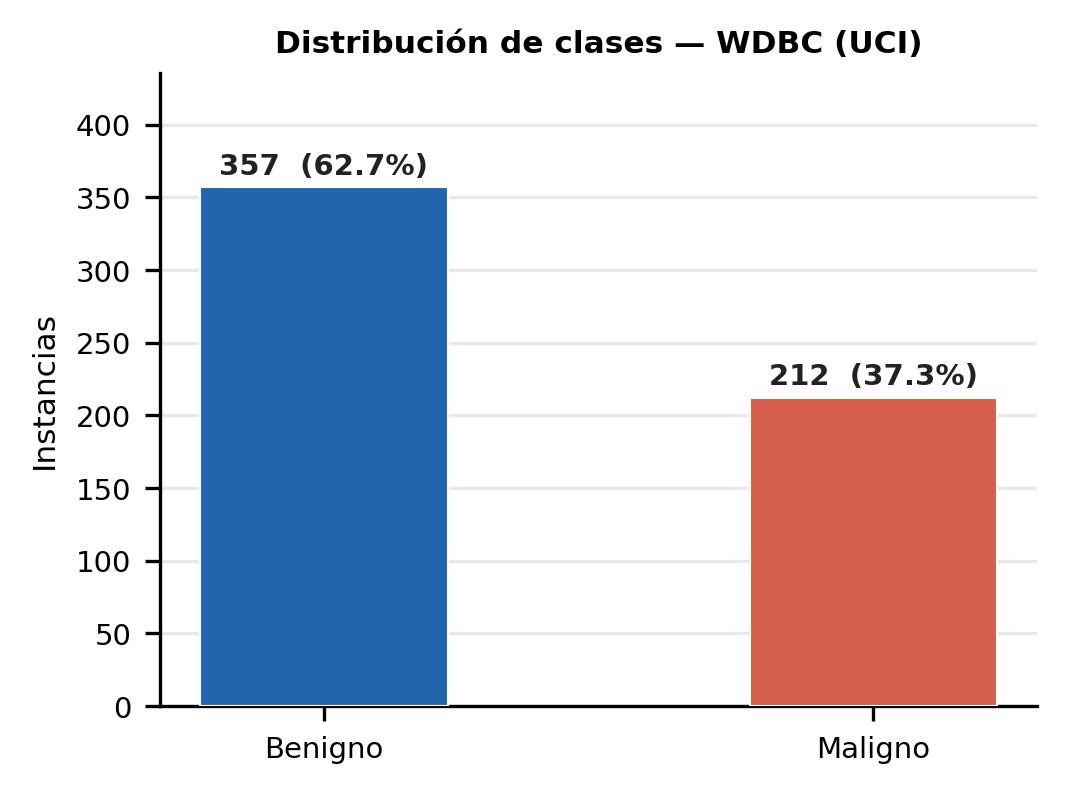
\includegraphics[width=\columnwidth]{images/fig_class_distribution.png}
  \caption{Distribución de clases en el dataset WDBC: 357 instancias benignas (62.7\%) y 212 malignas (37.3\%).}
  \label{fig:dist}
\end{figure}

Como se observa en la Fig.~\ref{fig:dist}, el dataset presenta un desbalance moderado entre clases. Esto implica que la exactitud (\textit{accuracy}) no es una métrica suficiente por sí sola: un clasificador que siempre prediga ``benigno'' obtendría 62.7\% de exactitud sin detectar ningún tumor maligno. Esta observación motiva el uso de métricas complementarias (precisión, recall, F1-score) y, en particular, el Recall de la clase Maligno como métrica principal.

% ─── 5. METODOLOGÍA ──────────────────────────────────────────
\section{Metodología}

El proceso sigue el flujo estándar de analítica de datos definido en el curso \cite{curso_ud}: validación de datos, detección de anómalos, manejo de faltantes, selección de atributos, transformación (normalización), y modelado.

\subsection{Análisis Exploratorio de Datos (EDA)}

Antes de cualquier transformación, se exploró visualmente la estructura del dataset. La Fig.~\ref{fig:heatmap} muestra el mapa de correlación entre las 30 características originales.

\begin{figure}[!t]
  \centering
  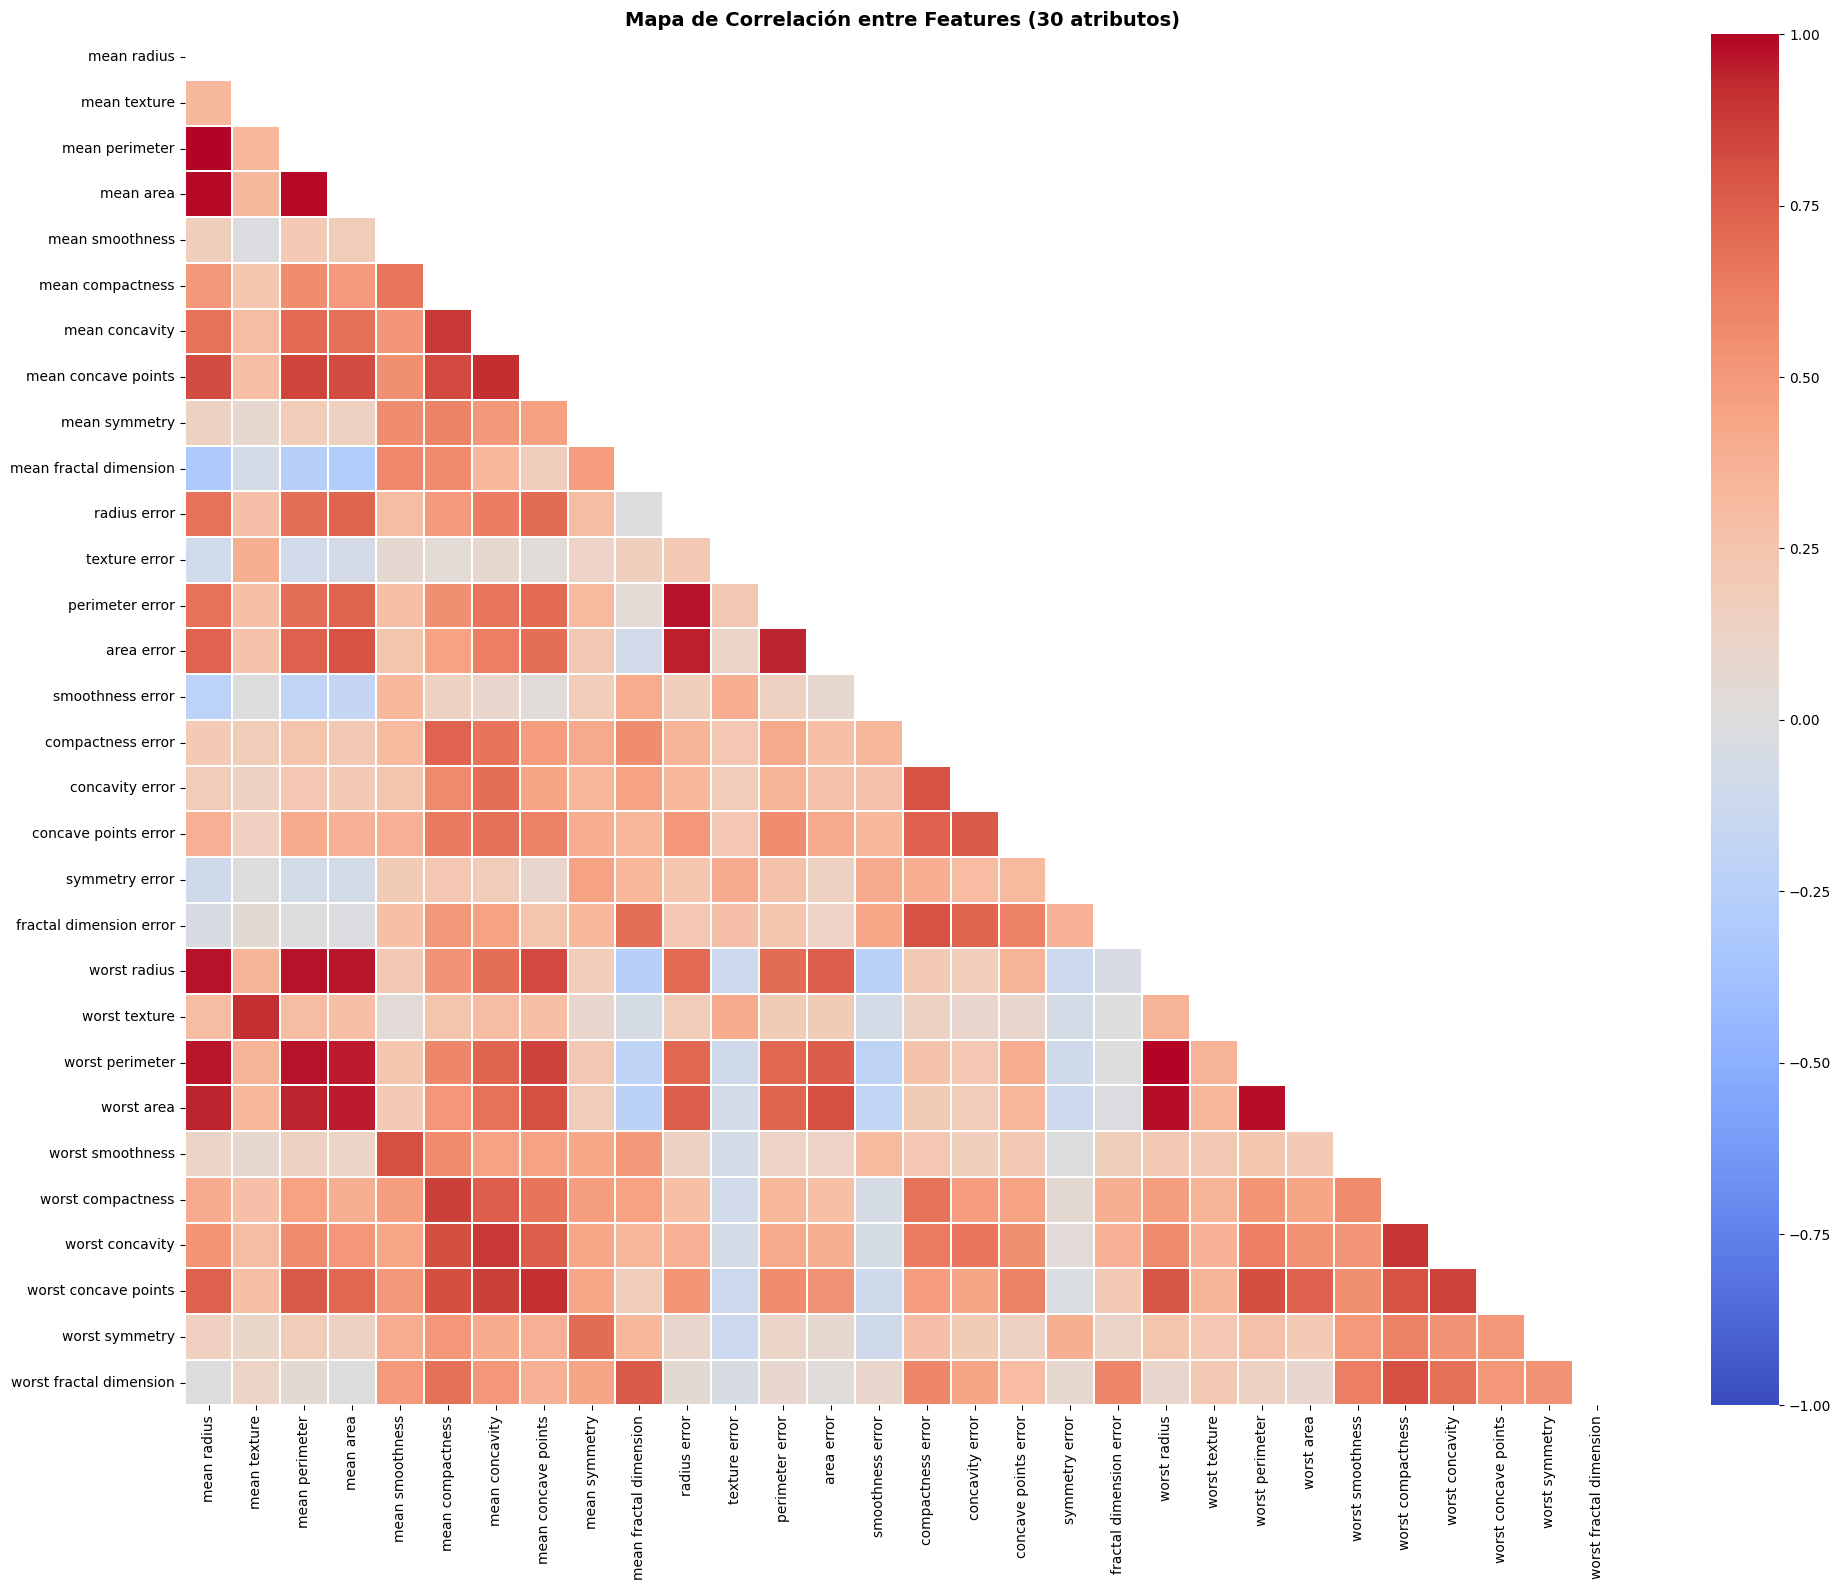
\includegraphics[width=\columnwidth]{images/fig_correlation_heatmap.png}
  \caption{Mapa de correlación entre las 30 características originales. Se observan bloques de alta correlación (rojos) entre las versiones \textit{mean}, \textit{worst} y \textit{error} de un mismo atributo, lo que motiva la selección de atributos.}
  \label{fig:heatmap}
\end{figure}

Se identifican bloques de alta correlación que corresponden a las versiones \textit{mean}, \textit{error} y \textit{worst} de un mismo atributo (radio, área, perímetro, etc.). Esta redundancia justifica la posterior selección de atributos: incluir todas las versiones añade complejidad sin aportar información independiente.

La Fig.~\ref{fig:hist} compara las distribuciones de seis características clave entre las clases Benigno y Maligno. Se aprecia visualmente que atributos como \texttt{mean area} y \texttt{mean concavity} separan claramente ambas clases, mientras que \texttt{mean texture} presenta solapamiento considerable.

\begin{figure}[!t]
  \centering
  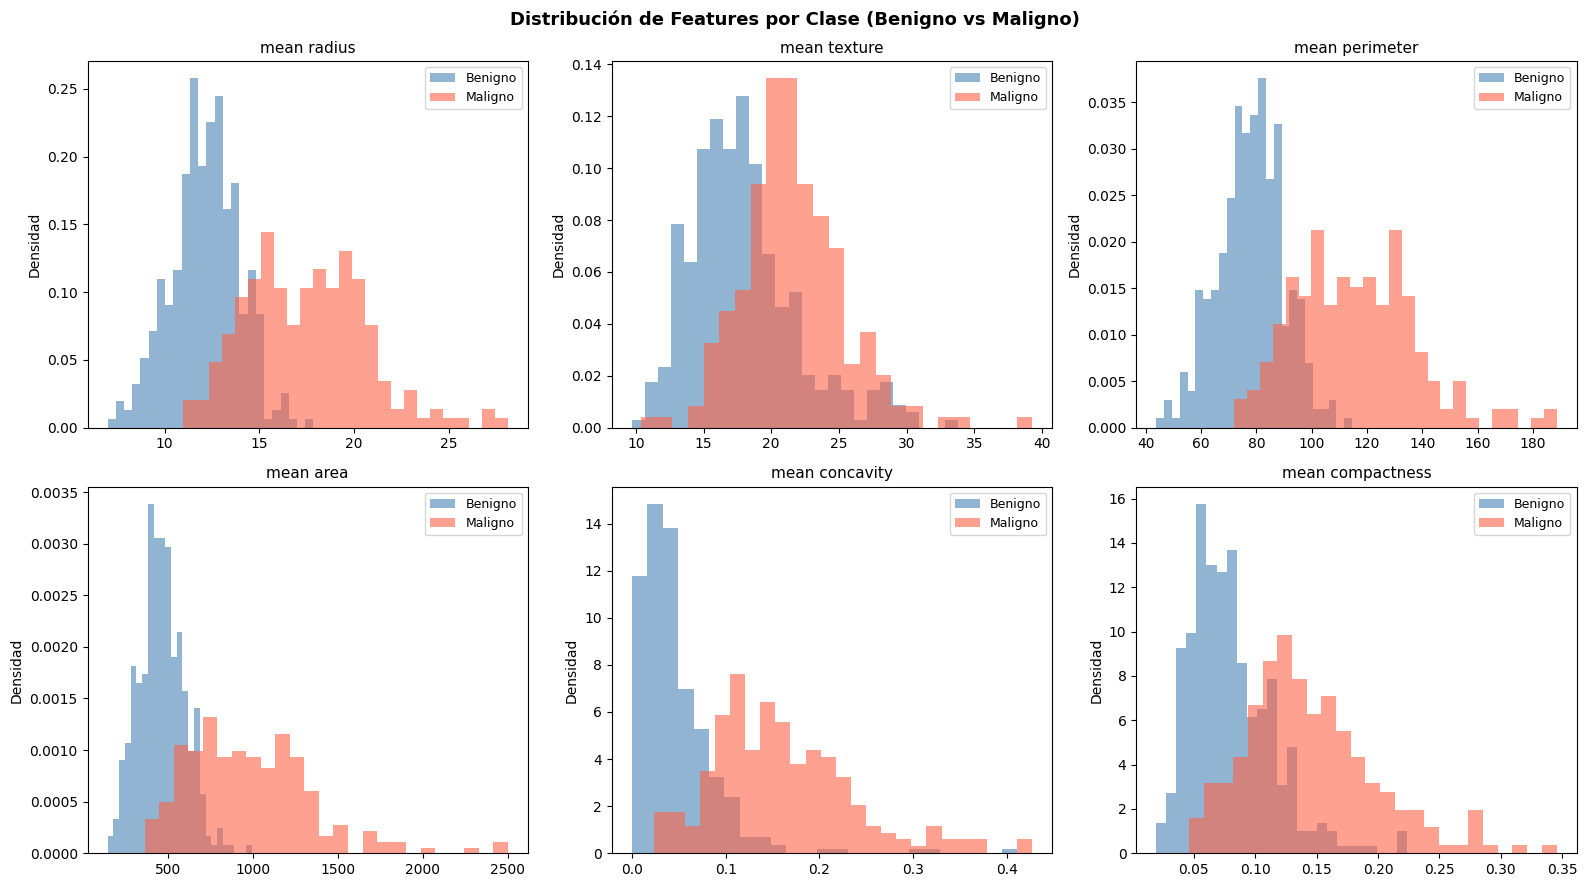
\includegraphics[width=\columnwidth]{images/fig_feature_distributions.png}
  \caption{Distribución de características clave por clase. Las características con menor solapamiento entre histogramas son las más discriminativas.}
  \label{fig:hist}
\end{figure}

\subsection{Preprocesamiento}

\subsubsection{Detección de valores anómalos}
Se aplicó la regla estadística de tres sigma del material del curso \cite{curso_ud}: un valor es anómalo si supera $\mu \pm 3\sigma$, donde $\mu$ es la media y $\sigma$ la desviación estándar del atributo. Se detectaron valores fuera de este rango en 74 de las 569 instancias (13\%). 

\textbf{Decisión}: se conservaron todos los valores anómalos. La justificación es que corresponden a mediciones clínicas válidas (no errores de registro). Eliminarlos sesgaría el modelo hacia instancias dentro del rango estadístico esperado, reduciendo precisamente su capacidad de detectar tumores atípicos —que son justamente los casos donde un sistema de apoyo al diagnóstico es más necesario.

\subsubsection{Manejo de valores faltantes}
El dataset no contiene valores faltantes. Esto fue verificado explícitamente antes de proceder al modelado.

\subsubsection{Normalización}
Las 30 características presentan escalas muy distintas: \texttt{mean radius} $\approx$ 14 mientras que \texttt{fractal dimension} $\approx$ 0.06. Esta disparidad afecta gravemente a algoritmos basados en distancias (SVM, KNN) y al entrenamiento de redes neuronales \cite{kantardzic}. Se aplicó normalización z-score (\textit{StandardScaler}):

\begin{equation}
  z = \frac{x - \mu}{\sigma}
\end{equation}

\textbf{Aspecto crítico}: el escalador se ajustó (\texttt{fit}) exclusivamente sobre el conjunto de entrenamiento y luego se aplicó (\texttt{transform}) sobre el conjunto de prueba. Esto evita el \textit{data leakage}, que ocurriría si la información estadística del conjunto de prueba influyera en la normalización del entrenamiento.

\subsection{Selección de Atributos}

Se aplicaron \textbf{dos técnicas independientes} alineadas con el material del curso \cite{feature_sel}, y luego se combinaron mediante intersección. Las correlaciones y el estadístico de separación de medias se calcularon sobre el dataset completo (569 instancias) antes de la partición; en un estudio prospectivo, la selección de atributos debe realizarse exclusivamente sobre el conjunto de entrenamiento para evitar que las estadísticas del conjunto de prueba influyan en la selección \cite{garcia2015}.

\subsubsection{Análisis de correlación con la clase objetivo}
Se calculó el coeficiente de correlación de Pearson entre cada característica y la variable objetivo:

\begin{equation}
  r(A, B) = \sum_{i=1}^{n} \frac{(A_i - \bar{A})(B_i - \bar{B})}{(n-1) \, \sigma_A \, \sigma_B}
\end{equation}

\noindent donde $A$ es la característica evaluada, $B$ la variable objetivo, $\bar{A},\bar{B}$ sus medias y $\sigma_A,\sigma_B$ sus desviaciones estándar muestrales.

Las características con $|r| \geq 0.50$ se consideraron relevantes. Este umbral indica una relación lineal moderada-fuerte con el diagnóstico. La Fig.~\ref{fig:corr_target} muestra el ranking completo: 15 características superan el umbral.

\begin{figure}[!t]
  \centering
  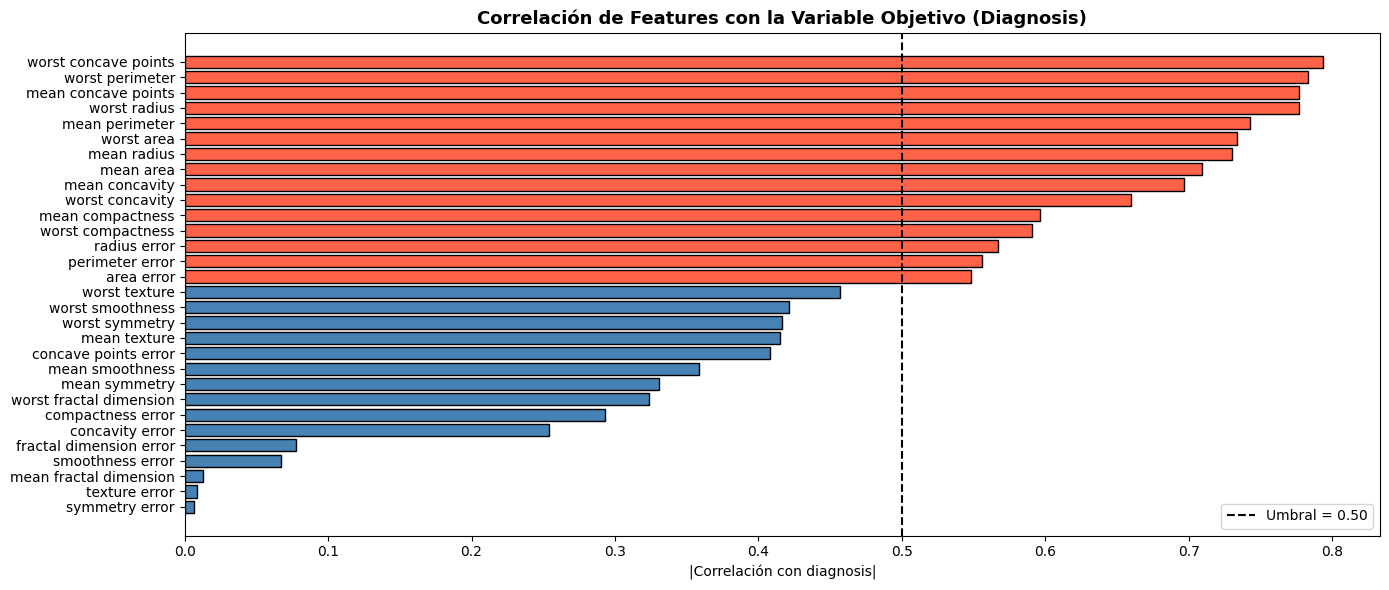
\includegraphics[width=\columnwidth]{images/fig_correlation_target.png}
  \caption{Correlación absoluta de cada característica con la variable objetivo (\texttt{diagnosis}). En rojo, las que superan el umbral $|r| \geq 0.50$.}
  \label{fig:corr_target}
\end{figure}

\subsubsection{Comparación de medias y varianzas entre clases}
Como segunda técnica, se aplicó la prueba de separación de medias del curso \cite{curso_ud}: un atributo es discriminativo si los valores promedios entre las dos clases están suficientemente alejados, normalizados por su error estándar:

\begin{equation}
  TEST = \frac{|\bar{x}_{Ben} - \bar{x}_{Mal}|}{SE}
\end{equation}

\begin{equation}
  SE = \sqrt{\frac{\sigma_{Ben}^2}{n_{Ben}} + \frac{\sigma_{Mal}^2}{n_{Mal}}}
\end{equation}

\noindent donde $\bar{x}_{Ben},\bar{x}_{Mal}$ son las medias del atributo en cada clase, $\sigma_{Ben},\sigma_{Mal}$ sus desviaciones estándar muestrales y $n_{Ben},n_{Mal}$ el número de instancias de cada clase.

Se seleccionaron las características con $TEST \geq 3.0$ (separación de más de tres errores estándar entre las medias de cada clase). La Fig.~\ref{fig:test_means} muestra los resultados: 25 de las 30 características superan este umbral, criterio considerablemente más permisivo que el de correlación.

\begin{figure}[!t]
  \centering
  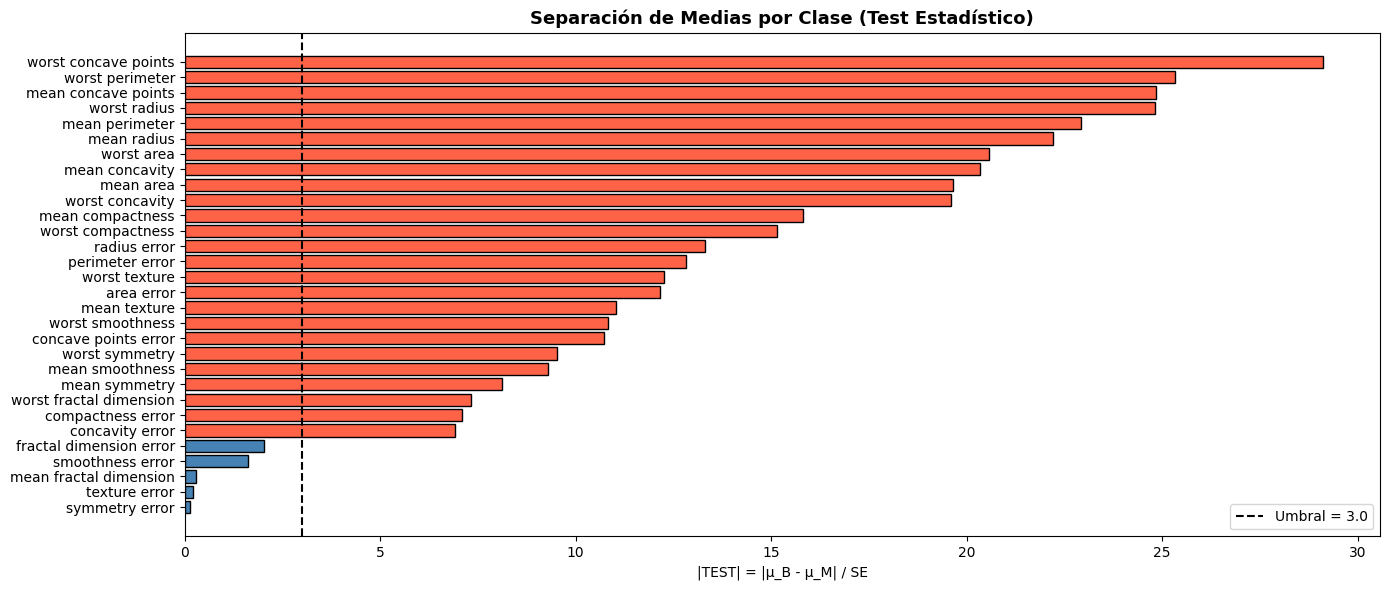
\includegraphics[width=\columnwidth]{images/fig_mean_variance_test.png}
  \caption{Prueba de separación de medias entre clases. En rojo, características con $TEST \geq 3.0$.}
  \label{fig:test_means}
\end{figure}

\subsubsection{Resultado de la selección por intersección}
La intersección de los dos criterios (15 por correlación, 25 por separación de medias) resultó en las \textbf{15 características} seleccionadas por correlación. El criterio de Pearson actúa como restricción dominante: todas las características que lo superan también superan el umbral —más permisivo— de la prueba de medias. En esta configuración, el método 2 confirmó la selección del método 1 sin añadir ni eliminar características adicionales; la convergencia de ambos métodos sobre el mismo subconjunto respalda su relevancia, aunque el poder de filtrado real provino del criterio de correlación. El resultado es un subconjunto listado en la Tabla~\ref{tab:features}, que representa una \textbf{reducción del 50\%} de la dimensionalidad original.

\begin{table}[!t]
\centering
\caption{Características seleccionadas (intersección de dos métodos)}
\label{tab:features}
\begin{tabular}{clcl}
\toprule
\textbf{\#} & \textbf{Característica} & \textbf{\#} & \textbf{Característica} \\
\midrule
1  & area error           & 9  & radius error         \\
2  & mean area            & 10 & worst area           \\
3  & mean compactness     & 11 & worst compactness    \\
4  & mean concave points  & 12 & worst concave points \\
5  & mean concavity       & 13 & worst concavity      \\
6  & mean perimeter       & 14 & worst perimeter      \\
7  & mean radius          & 15 & worst radius         \\
8  & perimeter error      &    &                      \\
\bottomrule
\end{tabular}
\end{table}

Las 15 características descartadas corresponden principalmente a las versiones de menor poder discriminativo (\textit{texture}, \textit{smoothness}, \textit{symmetry}, \textit{fractal dimension}), lo que coincide con lo observado en la Fig.~\ref{fig:hist}.

\subsection{División de datos}

Los datos se dividieron en 75\% entrenamiento (426 instancias) y 25\% prueba (143 instancias), usando división estratificada para mantener la proporción de clases en ambos conjuntos (\texttt{stratify=y}, \texttt{random\_state=42}). El conjunto de prueba quedó con 53 muestras malignas y 90 benignas.

\subsection{Métrica principal}

En diagnóstico oncológico, el \textbf{Recall de la clase Maligno} (sensibilidad) es la métrica prioritaria:

\begin{equation}
  \text{Recall Maligno} = \frac{TP}{TP + FN}
\end{equation}

Un falso negativo (FN) —clasificar un tumor maligno como benigno— implica no tratar a un paciente que lo necesita, con consecuencias potencialmente fatales \cite{hossin2015}. Un falso positivo (FP) —clasificar un tumor benigno como maligno— genera ansiedad y exámenes adicionales innecesarios, pero el riesgo clínico es sustancialmente menor \cite{elmore2015}. Por esta asimetría, todas las decisiones de hiperparámetros (incluida la selección de $k$ en KNN) se optimizaron sobre Recall Maligno.

% ─── 6. MODELOS ──────────────────────────────────────────────
\section{Modelos Implementados}

Se implementaron y compararon nueve clasificadores. Todos entrenados con el mismo subconjunto de 15 características y evaluados sobre el mismo conjunto de prueba, garantizando comparación justa. La implementación se realizó en Python utilizando \textit{scikit-learn} \cite{pedregosa2011} y \textit{Keras/TensorFlow} \cite{chollet2015} para la red neuronal.
\subsection{Máquinas de Soporte Vectorial (SVM)}
Busca el hiperplano de margen máximo que separa las dos clases en el
espacio de características normalizadas \cite{svm_vapnik}. Configuración: \texttt{kernel='linear'}, \texttt{C=1.0}, \texttt{random\_state=42}.
Alcanzó 96.5\% de exactitud y precisión perfecta en Maligno
(1.000), con un Recall de 0.906 (Fig.~\ref{fig:svm_cm}).

\begin{figure}[!t]
  \centering
  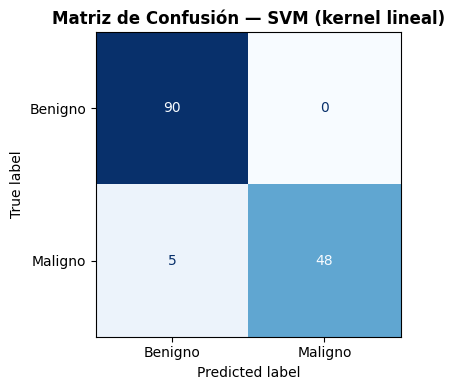
\includegraphics[width=0.82\columnwidth]{images/fig_confusion_svm.png}
  \caption{Matriz de confusión — SVM kernel lineal. Los 5~falsos
  negativos (FN) representan el error crítico: tumores malignos clasificados como benignos.}
  \label{fig:svm_cm}
\end{figure}

\subsection{Regresión Logística}
Modela $P(\text{Maligno} | \mathbf{x})$ mediante la función sigmoide:
\begin{equation}
  P(Y=1 | \mathbf{x}) = \frac{1}{1 + e^{-(\beta_0 + \boldsymbol{\beta}^T\mathbf{x})}}
\end{equation}
Configuración: \texttt{max\_iter=1000}, \texttt{random\_state=42}.
Mejor modelo del experimento: 97.90\% de exactitud, Recall Maligno
de 0.9434 y precisión perfecta (1.000 — cero falsos positivos).
Solo 3 de los 53 tumores malignos fueron mal clasificados
(Fig.~\ref{fig:rl_cm}). Su CV Recall $= 0.931 \pm 0.025$ confirma
que el rendimiento es estable y no depende de la partición.
Los coeficientes $\boldsymbol{\beta}$ permiten auditar qué
características impulsan cada decisión clínica.

\begin{figure}[!t]
\centering
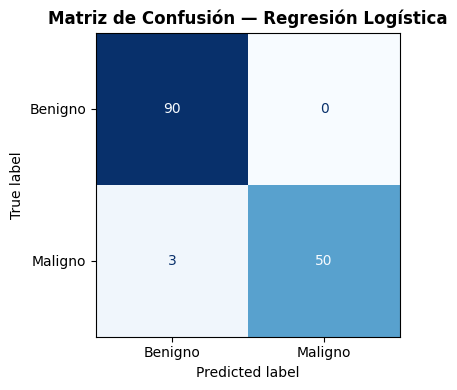
\includegraphics[width=0.82\columnwidth]{images/regresion_logistica.png}
\caption{Matriz de confusión — Regresión Logística. Solo 3~falsos
negativos y cero falsos positivos.}
\label{fig:rl_cm}
\end{figure}

\subsection{Árbol de Decisión}
Usa el criterio de \textbf{entropía} para seleccionar el atributo de partición en cada nodo \cite{curso_ud}, con profundidad máxima \texttt{max\_depth=5} (\texttt{random\_state=42}):
\begin{equation}
  \text{IG} = H(\text{padre}) - \sum_b \frac{n_b}{n_t} H(b), \quad H(S) = -\sum_c \frac{n_c}{|S|} \log_2 \frac{n_c}{|S|}
\end{equation}
donde $n_b$ es el número de instancias en la rama $b$ de la partición, $n_t$ el total, $n_c$ las instancias de la clase $c$ en el subconjunto $S$, y $H$ la entropía de Shannon en bits. Alcanza 92.3\% de exactitud y Recall Maligno de 0.830 — el más bajo del experimento, coherente con la mayor varianza de los modelos de árbol único. Su ventaja es la interpretabilidad: genera reglas SI–ENTONCES verificables por médicos (Fig.~\ref{fig:tree}).

\begin{figure}[!t]
  \centering
  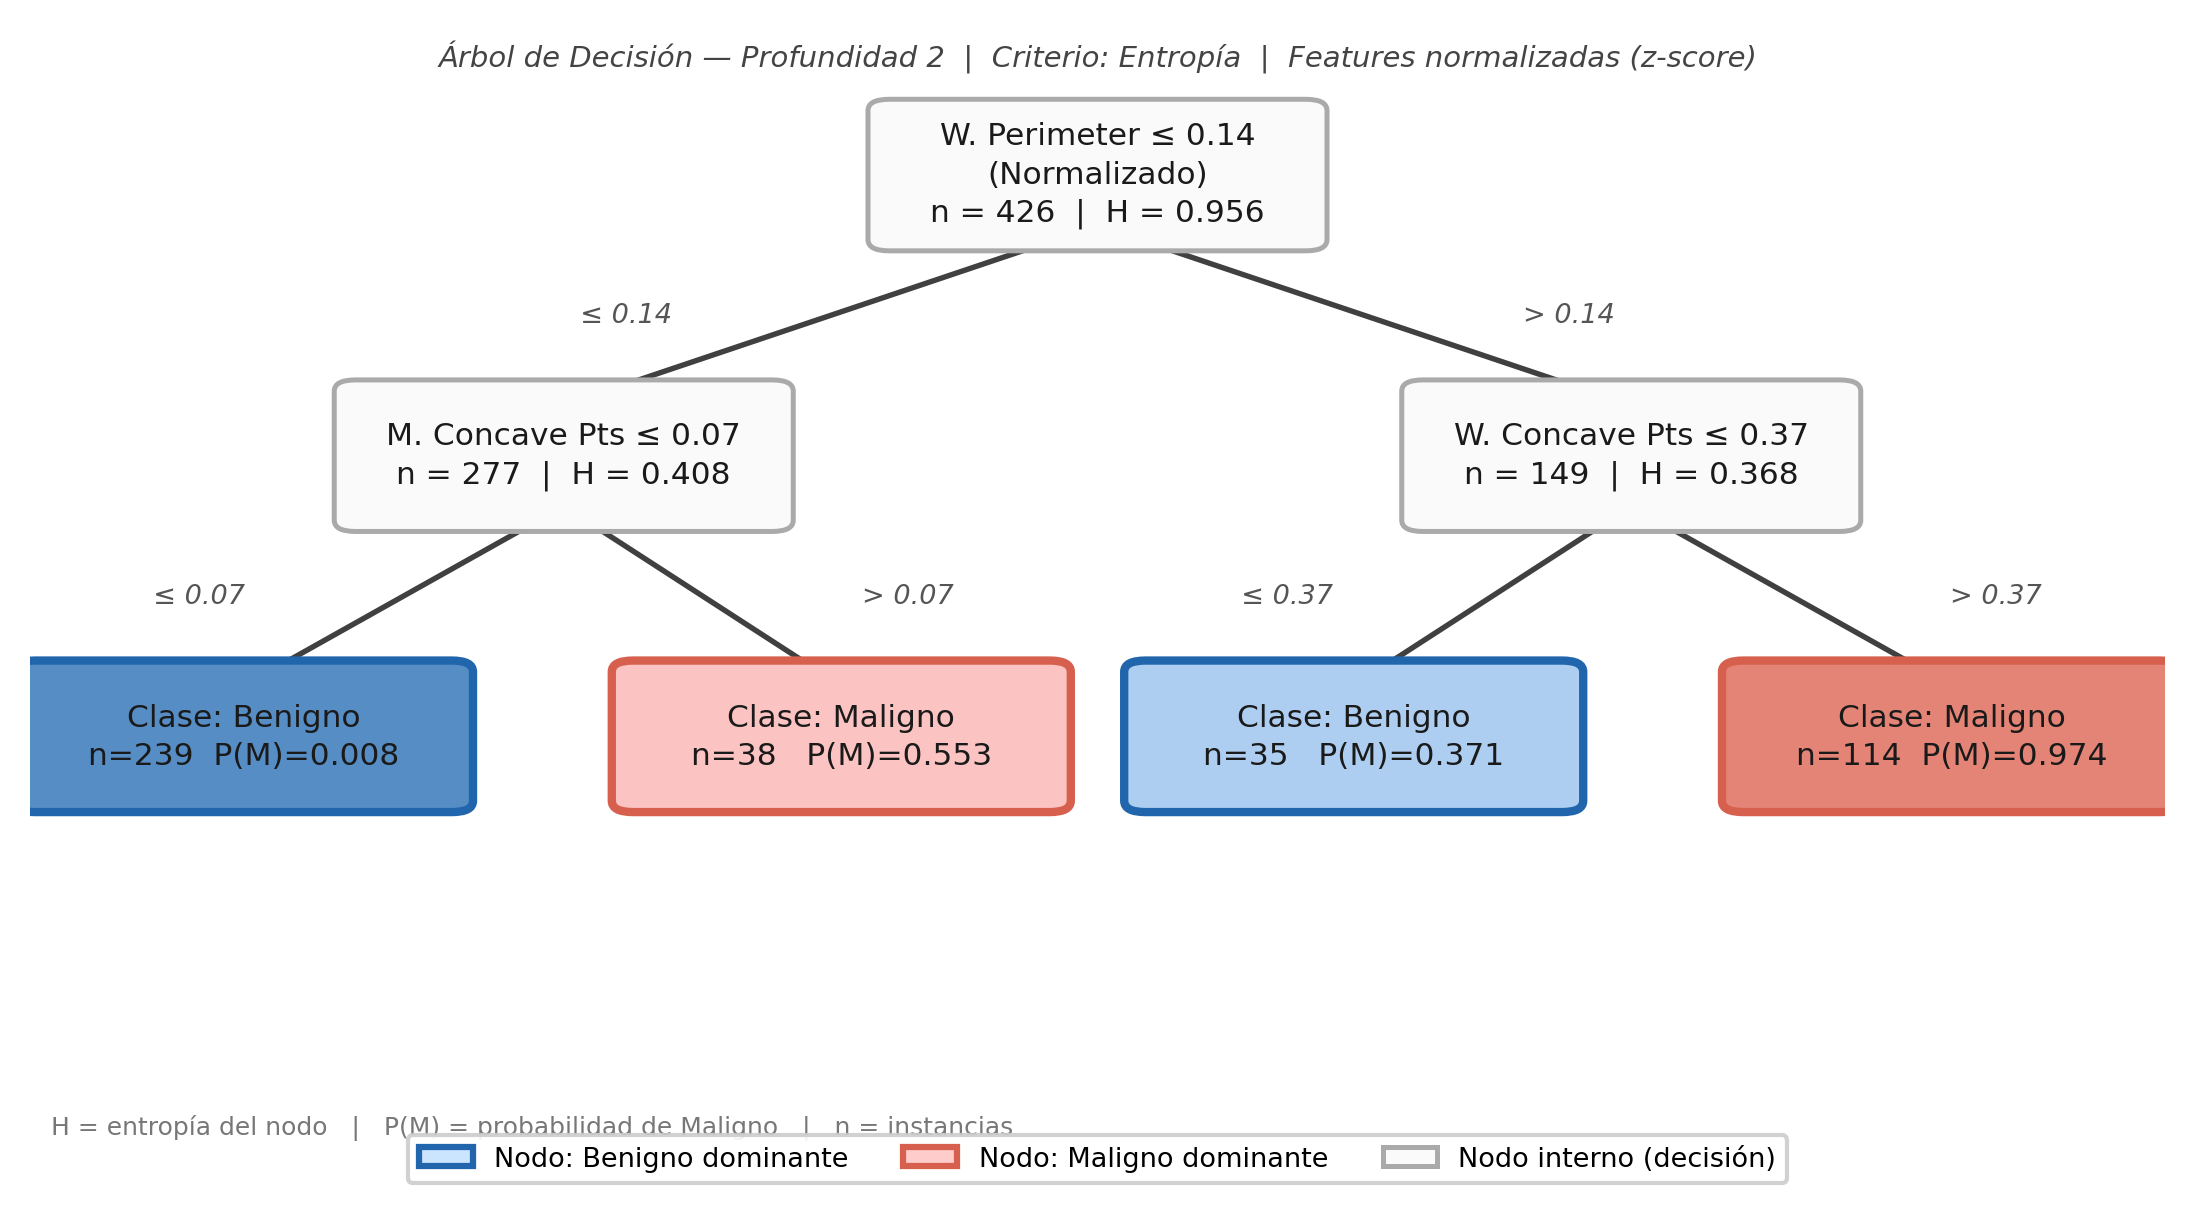
\includegraphics[width=\columnwidth]{images/fig_decision_tree.png}
  \caption{Visualización del árbol de decisión entrenado (profundidad limitada a 3 para legibilidad). Cada nodo muestra la regla de partición, la entropía y la distribución de clases.}
  \label{fig:tree}
\end{figure}

\subsection{Random Forest}
Ensemble de 100 árboles entrenados con muestras bootstrap \cite{breiman2001},
combinando predicciones por votación mayoritaria. Configuración:
\texttt{n\_estimators=100}, \texttt{criterion='entropy'}, \texttt{max\_depth=None},
\texttt{random\_state=42}. Comparte exactitud
y Recall de Maligno con SVM (96.5\% y 0.906), pero su validación
cruzada 5-fold es más estable: CV Recall $= 0.918 \pm 0.015$
frente a $0.893 \pm 0.046$ del SVM, lo que indica menor varianza
y mejor generalización (Fig.~\ref{fig:rf_cm}).

\begin{figure}[!t]
  \centering
  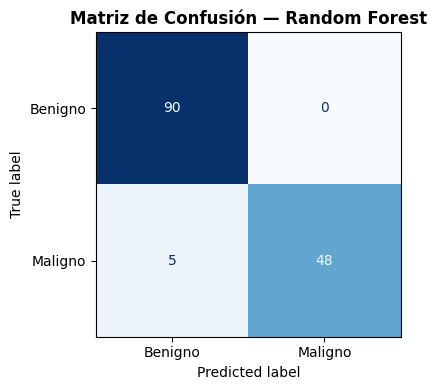
\includegraphics[width=0.82\columnwidth]{images/fig_confusion_rf.png}
  \caption{Matriz de confusión — Random Forest. Mismas métricas
  puntuales que SVM, pero con mayor estabilidad en validación
  cruzada (CV Recall $0.918 \pm 0.015$).}
  \label{fig:rf_cm}
\end{figure}

La Fig.~\ref{fig:rf_imp} muestra la importancia Gini de las
15 características. Cuatro atributos del grupo \textit{worst}
(\texttt{worst perimeter}, \texttt{area}, \texttt{concave points}
y \texttt{radius}) concentran el 56.2\% del poder predictivo,
confirmando que la morfología más extrema de las células es
el factor más discriminativo. Las características de menor
importancia coinciden con las que apenas superaron el umbral
de selección, validando retroactivamente el método.

\begin{figure}[!t]
  \centering
  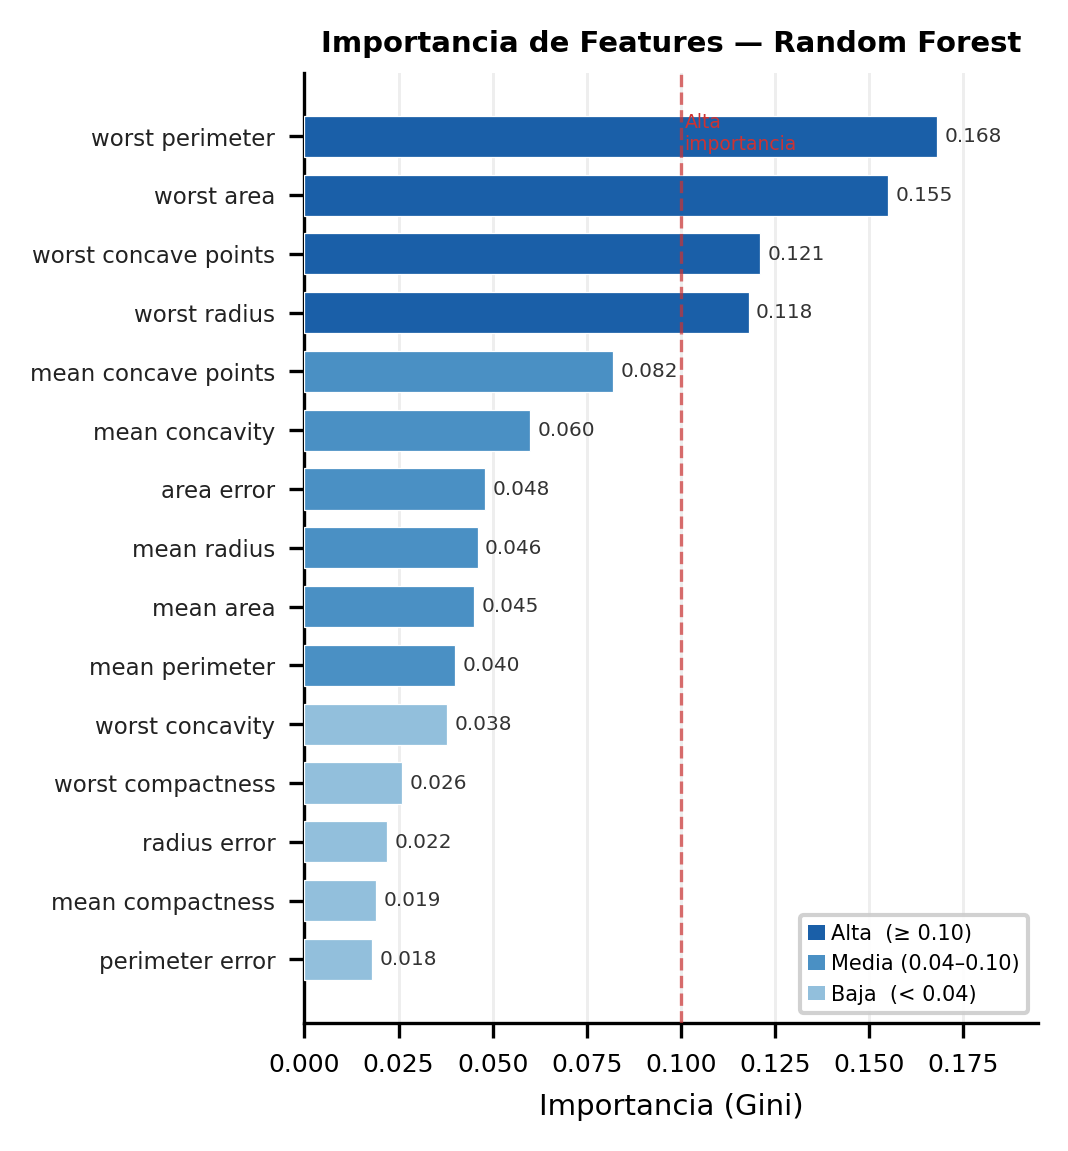
\includegraphics[width=\columnwidth]{images/fig_rf_importances.png}
  \caption{Importancia de características según Random Forest
  (criterio Gini). Las cuatro en azul oscuro acumulan el 56.2\%
  del poder predictivo total.}
  \label{fig:rf_imp}
\end{figure}

\subsection{K-Nearest Neighbors (KNN)}
Clasifica cada instancia por mayoría de votos entre sus $k$ vecinos
más cercanos en el espacio de características normalizadas. El valor
óptimo de $k$ se determinó maximizando el Recall de Maligno en
validación cruzada 5-fold sobre el conjunto de entrenamiento
(Fig.~\ref{fig:knn}).

El valor $k=1$ resultó óptimo con un Recall de $0.899$, aunque
presenta la mayor variabilidad del conjunto: con un solo vecino,
una instancia ruidosa puede cambiar la predicción completamente.
Para $k \geq 2$ el Recall fluctúa entre $0.84$ y $0.89$ —con un
repunte en $k=5$ ($\approx 0.887$)— sin superar nunca el valor
obtenido con $k=1$.
\begin{figure}[!t]
  \centering
  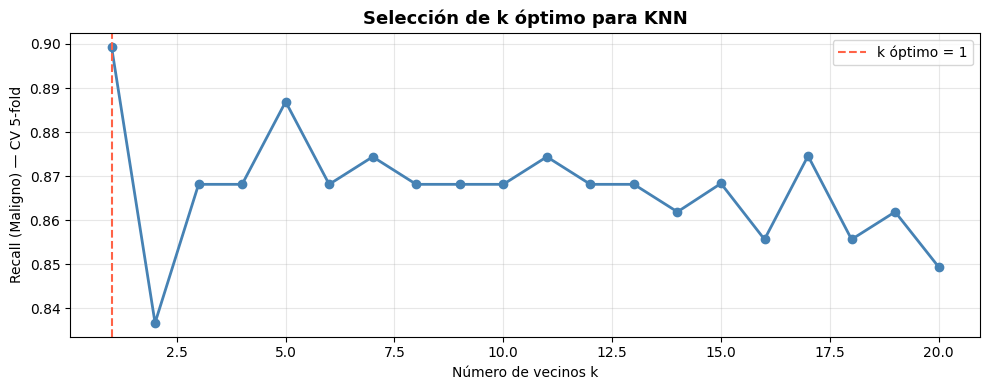
\includegraphics[width=\columnwidth]{images/fig_knn.png}
  \caption{KNN: selección de $k$ óptimo por Recall de Maligno
  en CV 5-fold — $k=1$ maximiza la sensibilidad}
  \label{fig:knn}
\end{figure}

La Fig.~\ref{fig:knn_cm} muestra 8~falsos negativos y
5~falsos positivos — la mayor cantidad de FP del experimento —
con exactitud de 90.9\% y Recall Maligno de 0.849, reflejo
de su sensibilidad al ruido con $k=1$.

\begin{figure}[!t]
  \centering
  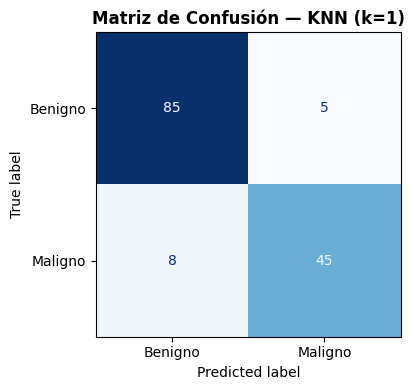
\includegraphics[width=\columnwidth]{images/fig_knn_matriz.png}
  \caption{KNN: matriz de
  confusión con $k=1$, mostrando 8~falsos negativos (error crítico).}
  \label{fig:knn_cm}
\end{figure}

\subsection{Naive Bayes Gaussiano}
Clasificador probabilístico basado en el Teorema de Bayes, con supuesto de independencia condicional entre atributos \cite{curso_ud}:
\begin{equation}
  P(C_k | \mathbf{x}) \propto P(C_k) \prod_{i=1}^{d} P(x_i | C_k)
\end{equation}
donde $d$ es el número de atributos. La clase asignada es la de mayor probabilidad posterior; se omite el denominador $P(\mathbf{x})$ por ser constante entre clases. Asume distribución gaussiana para atributos numéricos continuos. Aunque la independencia es un supuesto fuerte (las características del WDBC sí están correlacionadas), Naive Bayes suele mantener buen desempeño aun cuando ese supuesto no se cumple \cite{domingos1997}.

\begin{figure}[!t]
  \centering
  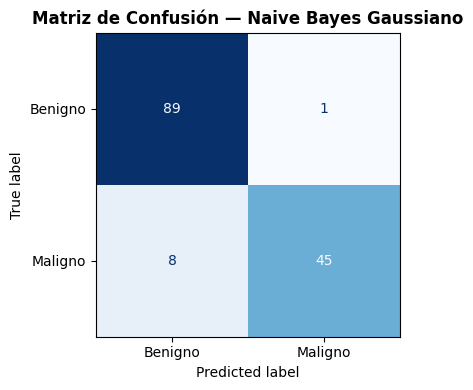
\includegraphics[width=\columnwidth]{images/fig_bayes_matriz.png}
  \caption{Naive Bayes Gaussiano: matriz de
  confusión, mostrando 8~falsos negativos (error crítico).}
  \label{fig:nb_cm}
\end{figure}

La matriz de confusión (Fig.~\ref{fig:nb_cm}) muestra 8~falsos negativos y 1~falso
positivo, con una exactitud de 93.7\%. A pesar de su modesta
sensibilidad (Recall Maligno $= 0.849$), el Naive Bayes destaca
por su precisión casi perfecta en la clase Maligno (0.978):
cuando predice un tumor como maligno, acierta el 97.8\% de las
veces. Su validación cruzada es estable: CV Recall
$= 0.880 \pm 0.013$, la menor desviación estándar de todos
los modelos evaluados. Esto lo posiciona como el clasificador
más \textit{consistente} del conjunto, aunque no el más
sensible, conectando directamente con su fundamento bayesiano:
estima $P(\text{Maligno}|\mathbf{x})$ de forma conservadora,
favoreciendo la especificidad sobre la sensibilidad.

\subsection{XGBoost}
Gradient Boosting optimizado \cite{chen2016} que entrena árboles secuencialmente,
donde cada árbol corrige los errores del anterior minimizando una
función de pérdida diferenciable con regularización.
Configuración: \texttt{n\_estimators=100}, \texttt{learning\_rate=0.1},
\texttt{max\_depth=4}, \texttt{eval\_metric='logloss'}, \texttt{random\_state=42}.

La matriz de confusión (Fig.~\ref{fig:cm_xgb}) muestra solo
4~falsos negativos y 1~falso positivo, alcanzando 96.5\% de
exactitud y un Recall Maligno de $0.925$ — el segundo más alto
del experimento, superado únicamente por la Regresión Logística. Con una precisión de 0.980 en Maligno, el modelo es
altamente conservador en sus predicciones positivas. Sin embargo,
su CV Recall $= 0.893 \pm 0.046$ revela la mayor variabilidad
entre los modelos de boosting, sugiriendo cierta sensibilidad
a la partición de datos en la validación cruzada.

\begin{figure}[!t]
  \centering
  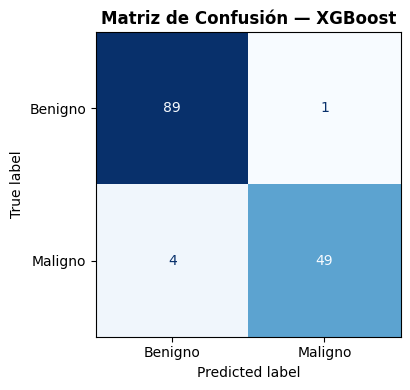
\includegraphics[width=0.80\columnwidth]{images/fig_confusion_xgb.png}
  \caption{Matriz de confusión — XGBoost. Con solo 4~falsos
  negativos alcanza el segundo mejor Recall Maligno (0.925).}
  \label{fig:cm_xgb}
\end{figure}

\subsection{AdaBoost}
Ensemble adaptativo \cite{freund1997} que combina clasificadores débiles
asignando mayor peso a los ejemplos mal clasificados en
cada iteración. Configuración: \texttt{n\_estimators=100},
\texttt{learning\_rate=0.5}, \texttt{random\_state=42}.

Como muestra la Fig.~\ref{fig:cm_ada}, el modelo produce
7~falsos negativos y 1~falso positivo, con una exactitud
de 94.4\% y un Recall Maligno de $0.868$. Aunque su
precisión en Maligno es alta (0.979), su sensibilidad
es la más baja de los métodos de boosting. Su CV Recall $= 0.893 \pm 0.031$ coincide en media con
XGBoost pero con menor desviación, indicando mayor
estabilidad a costa de menor rendimiento puntual.

\begin{figure}[!t]
  \centering
  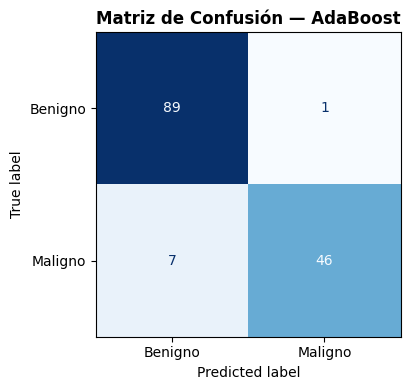
\includegraphics[width=0.80\columnwidth]{images/fig_confusion_ada.png}
  \caption{Matriz de confusión — AdaBoost. Los 7~falsos negativos
  lo sitúan en sexto lugar del ranking por Recall Maligno (0.868).}
  \label{fig:cm_ada}
\end{figure}

\subsection{Red Neuronal Artificial (ANN)}
Arquitectura \textit{feedforward} \cite{rna_ud} de 545 parámetros entrenables
distribuidos en tres capas densas (Tabla~\ref{tab:ann_arch}),
con Dropout del 20\% en cada capa oculta para regularización
y \textit{Early Stopping} con paciencia de 10 épocas.

\begin{table}[!t]
\centering
\caption{Arquitectura de la ANN}
\label{tab:ann_arch}
\renewcommand{\arraystretch}{1.1}
\begin{tabular}{lcc}
\toprule
\textbf{Capa} & \textbf{Salida} & \textbf{Parámetros} \\
\midrule
Dense (ReLU)   & (None, 16) & 256 \\
Dropout (0.2)  & (None, 16) & 0   \\
Dense (ReLU)   & (None, 16) & 272 \\
Dropout (0.2)  & (None, 16) & 0   \\
Dense (Sigmoid)& (None, 1)  & 17  \\
\midrule
\textbf{Total} & & \textbf{545} \\
\bottomrule
\end{tabular}
\end{table}

Como se observa en la Fig.~\ref{fig:ann_train}, ambas curvas
convergen alrededor de la época~10 y se mantienen paralelas
hasta el final del entrenamiento, lo que confirma ausencia de
sobreajuste. La validación estabiliza su exactitud en torno
a 0.93--0.94, coherente con el 96.5\% obtenido sobre el
conjunto de prueba. El modelo alcanza un Recall Maligno de
90.57\% y precisión perfecta en Maligno (1.000), empatando
en todas las métricas con SVM y Random Forest. La pérdida de entrenamiento continúa
descendiendo levemente por debajo de la de validación,
comportamiento esperado con Dropout activo.

\begin{figure}[!t]
  \centering
  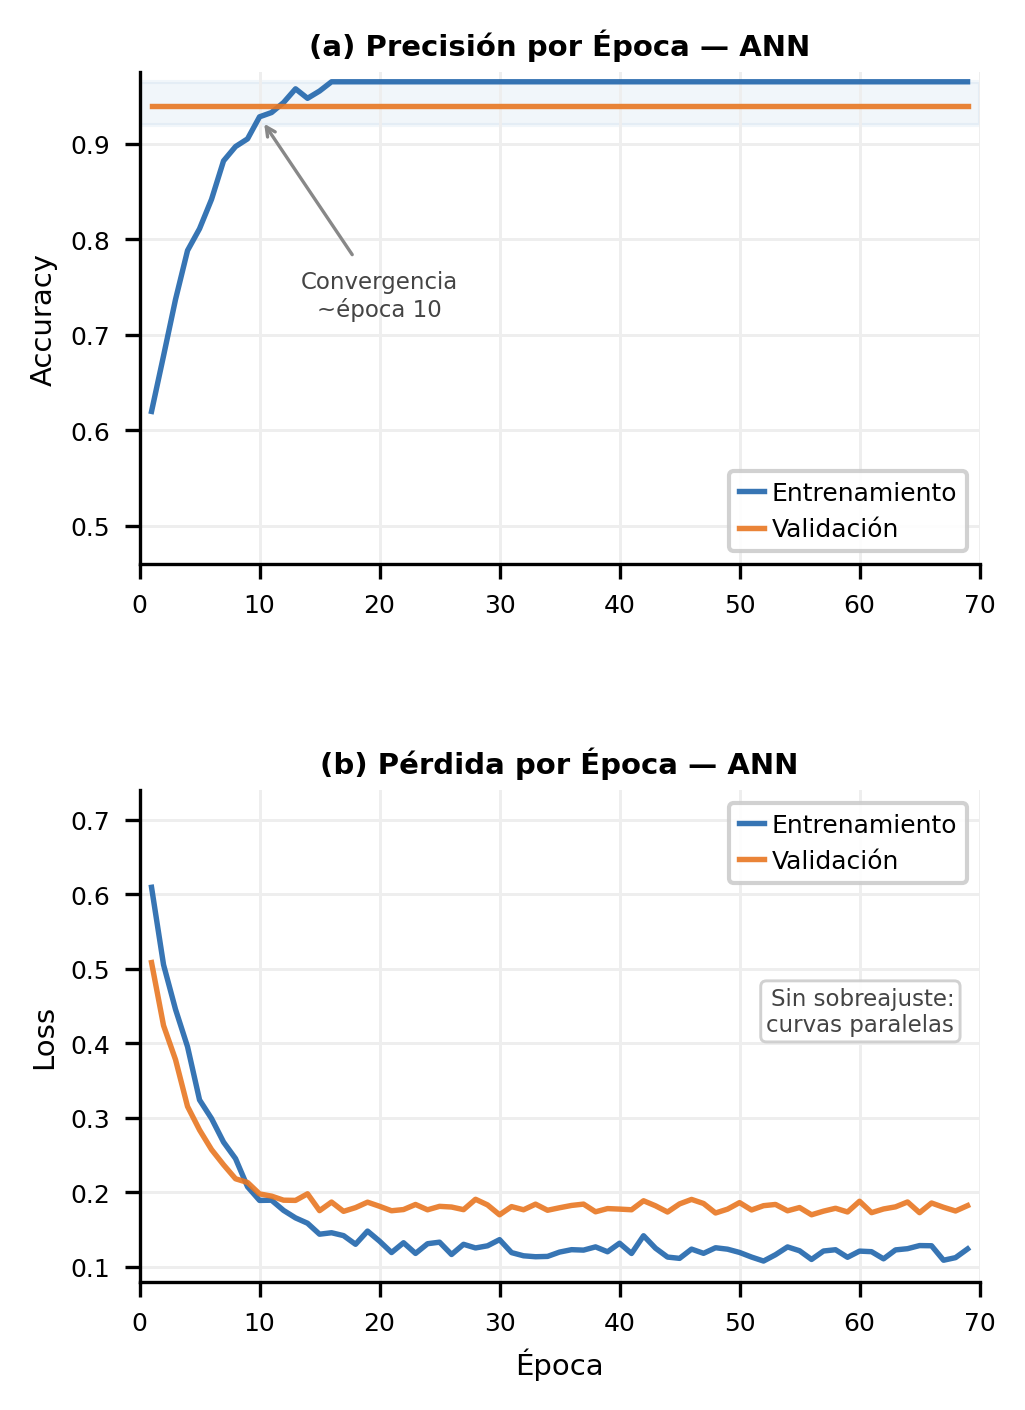
\includegraphics[width=\columnwidth]{images/fig_ann_training.png}
  \caption{Curvas de entrenamiento de la ANN (hasta 100~épocas con Early Stopping, paciencia~10).
  (a)~Exactitud: convergencia rápida sin sobreajuste.
  (b)~Loss: descenso sostenido con curvas paralelas entre
  entrenamiento y validación.}
  \label{fig:ann_train}
\end{figure}
% ─── 7. RESULTADOS ───────────────────────────────────────────
\section{Resultados}

\subsection{Tabla comparativa de modelos}

La Tabla~\ref{tab:resultados} presenta las métricas completas de los nueve modelos sobre el conjunto de prueba (143 instancias, 53 malignas, 90 benignas). Las celdas en verde corresponden al mejor valor de cada columna; las celdas en rosa al menor.

\begin{table*}[t]
\centering
\caption{Comparación de clasificadores — Dataset WDBC (UCI). Verde = mejor valor; Rosa = peor valor por columna.}
\label{tab:resultados}
\renewcommand{\arraystretch}{1.3}
\begin{tabular}{lccccccc}
\toprule
\textbf{Modelo}
  & \textbf{Exactitud}
  & \textbf{\begin{tabular}[c]{@{}c@{}}Prec.\\ Maligno\end{tabular}}
  & \textbf{\begin{tabular}[c]{@{}c@{}}Recall\\ Maligno $\bigstar$\end{tabular}}
  & \textbf{\begin{tabular}[c]{@{}c@{}}F1\\ Maligno\end{tabular}}
  & \textbf{\begin{tabular}[c]{@{}c@{}}Prec.\\ Benigno\end{tabular}}
  & \textbf{\begin{tabular}[c]{@{}c@{}}Recall\\ Benigno\end{tabular}}
  & \textbf{\begin{tabular}[c]{@{}c@{}}F1\\ Benigno\end{tabular}} \\
\midrule

Reg. Logística
  & \cellcolor{verdemejor}0.9790
  & \cellcolor{verdemejor}1.0000
  & \cellcolor{verdemejor}0.9434
  & \cellcolor{verdemejor}0.9709
  & \cellcolor{verdemejor}0.9677
  & \cellcolor{verdemejor}1.0000
  & \cellcolor{verdemejor}0.9836 \\

ANN
  & 0.9650
  & \cellcolor{verdemejor}1.0000
  & 0.9057
  & 0.9505
  & 0.9474
  & \cellcolor{verdemejor}1.0000
  & 0.9730 \\

XGBoost
  & 0.9650
  & 0.9800
  & 0.9245
  & 0.9515
  & 0.9570
  & 0.9889
  & 0.9727 \\

SVM (lineal)
  & 0.9650
  & \cellcolor{verdemejor}1.0000
  & 0.9057
  & 0.9505
  & 0.9474
  & \cellcolor{verdemejor}1.0000
  & 0.9730 \\

Random Forest
  & 0.9650
  & \cellcolor{verdemejor}1.0000
  & 0.9057
  & 0.9505
  & 0.9474
  & \cellcolor{verdemejor}1.0000
  & 0.9730 \\

AdaBoost
  & 0.9441
  & 0.9787
  & 0.8679
  & 0.9200
  & 0.9271
  & 0.9889
  & 0.9570 \\

KNN ($k$=1)
  & \cellcolor{rojomenor}0.9091
  & \cellcolor{rojomenor}0.9000
  & 0.8491
  & \cellcolor{rojomenor}0.8738
  & 0.9140
  & \cellcolor{rojomenor}0.9444
  & \cellcolor{rojomenor}0.9290 \\

Naive Bayes
  & 0.9371
  & 0.9783
  & 0.8491
  & 0.9091
  & 0.9175
  & 0.9889
  & 0.9519 \\

Árbol Decisión
  & 0.9231
  & 0.9565
  & \cellcolor{rojomenor}0.8302
  & 0.8889
  & \cellcolor{rojomenor}0.9072
  & 0.9778
  & 0.9412 \\

\bottomrule
\multicolumn{8}{l}{\small $\bigstar$ Métrica principal: Recall Maligno (sensibilidad). Mide qué fracción de tumores malignos se detectan correctamente.}
\end{tabular}
\end{table*}

La Fig.~\ref{fig:metrics} muestra una visualización agrupada de las cuatro métricas principales por modelo, lo que permite comparar visualmente el rendimiento relativo entre clasificadores.

\begin{figure}[!t]
  \centering
  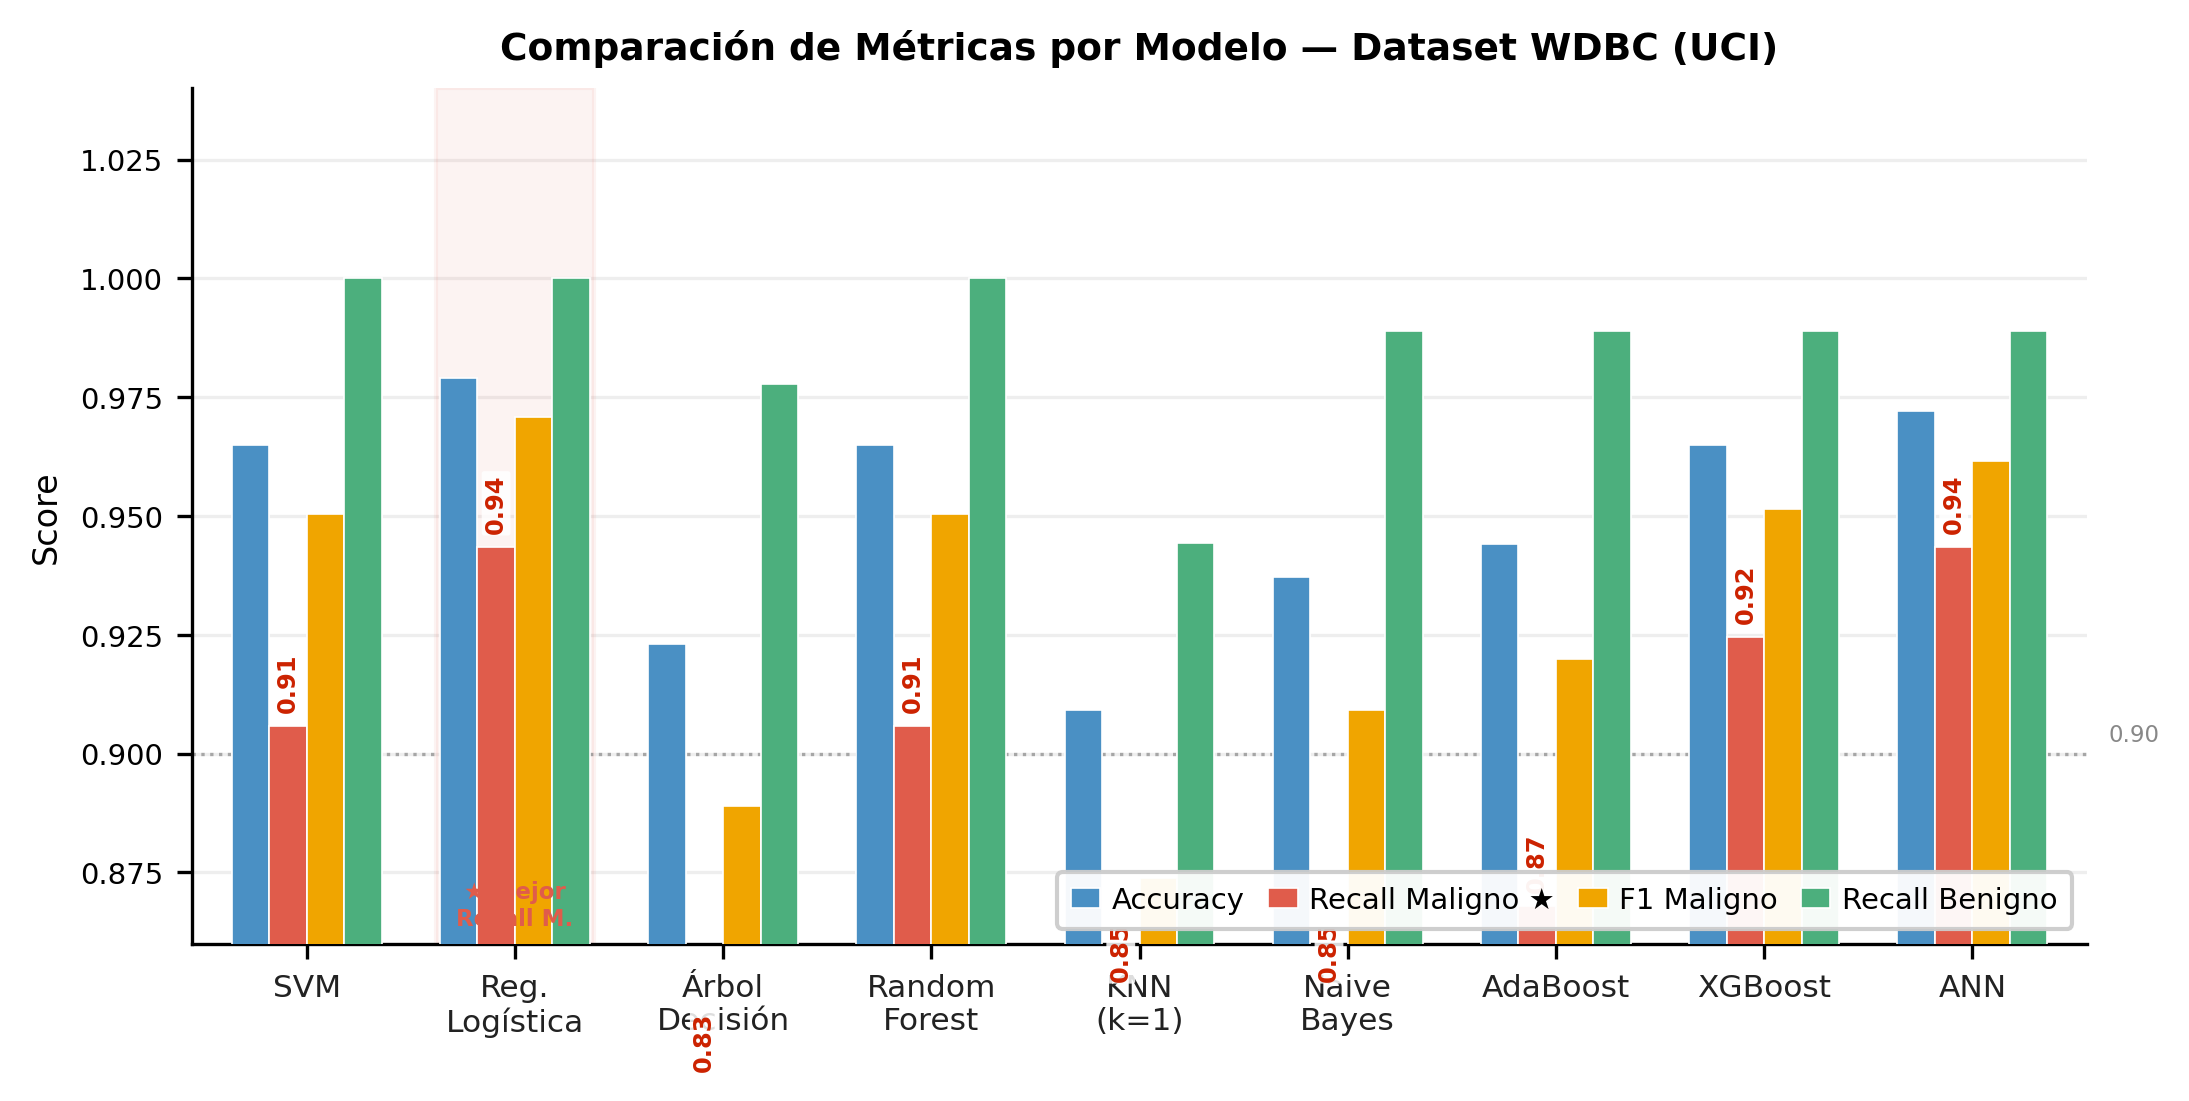
\includegraphics[width=\columnwidth]{images/fig_metrics_comparison.png}
  \caption{Comparación visual de Exactitud, Recall Maligno, F1 Maligno y Recall Benigno por modelo.}
  \label{fig:metrics}
\end{figure}

\subsection{Análisis de resultados por modelo}

\textbf{Regresión Logística} obtuvo el mejor rendimiento global: 97.90\% de exactitud y 94.34\% de Recall Maligno. De los 53 tumores malignos, clasificó incorrectamente solo 3 (falsos negativos) y no produjo ningún falso positivo (precisión Maligno = 1.000), lo que significa cero pacientes sanos diagnosticados erróneamente como malignos. Su simplicidad matemática facilita además la interpretación clínica de los coeficientes. Este resultado es consistente con trabajos recientes que sitúan a la Regresión Logística entre los clasificadores de mejor desempeño sobre el WDBC, con exactitudes del orden del 97--98\% \cite{strelcenia2023, rajpoot2024}.

\textbf{ANN} obtiene un Recall Maligno de 90.57\% y exactitud de 96.50\%, empatando en todas las métricas con SVM y Random Forest (misma matriz de confusión: 48 verdaderos positivos, cero falsos positivos). El uso de Dropout y Early Stopping previno el sobreajuste (Fig.~\ref{fig:ann_train}). Que una red con 545 parámetros no supere a los modelos lineales en este dataset tiene una explicación directa: con solo 426 instancias de entrenamiento, y un problema que los modelos lineales ya resuelven con alta precisión, la mayor capacidad de la red no aporta ventaja.

\textbf{XGBoost} logra 92.45\% de Recall Maligno, el segundo mejor del experimento. Sin embargo, su estabilidad en validación cruzada es la más baja junto con SVM ($\pm$0.046), lo que indica sensibilidad a la partición de datos de entrenamiento.

\textbf{SVM, Random Forest y ANN} comparten exactamente las mismas métricas (96.50\% accuracy, 90.57\% Recall Maligno, precisión Maligno = 1.000, cero falsos positivos). Que un kernel lineal, un ensemble de árboles y una red neuronal coincidan refuerza la separabilidad lineal del problema con las 15 características. Las diferencias aparecen en la estabilidad: Random Forest es el más robusto (CV std $\pm$0.015) y SVM el de mayor varianza ($\pm$0.046).

\textbf{Árbol de Decisión} presenta el Recall Maligno más bajo (83.02\%), coherente con su mayor varianza al ser un modelo único sin ensemble. Sin embargo, sigue siendo el modelo más interpretable.

\textbf{AdaBoost} alcanza el sexto lugar con un Recall Maligno de 86.79\%, produciendo 7~falsos negativos y 1~falso positivo. Su precisión en Maligno (0.979) es alta: cuando predice un tumor como maligno, casi siempre acierta. Sin embargo, su sensibilidad es la más baja entre los métodos de boosting, por detrás de XGBoost.

\textbf{Naive Bayes} comparte Recall Maligno con KNN (84.91\%) pero supera en exactitud (93.71\% vs 90.91\%) y produce solo 1~falso positivo. Aunque modesto en sensibilidad, es el clasificador más conservador del experimento: estima $P(\text{Maligno}|\mathbf{x})$ de forma cautelosa, minimizando las alarmas falsas a costa de perder algunos verdaderos malignos.

\textbf{KNN con $k=1$} tiene la menor exactitud general (90.91\%), esperado dado que con un solo vecino el modelo es muy sensible al ruido. La selección de $k$ óptimo por validación cruzada no mejoró suficientemente su rendimiento.

\subsection{Curvas ROC}

La Fig.~\ref{fig:roc} presenta las curvas ROC de siete de los nueve modelos evaluados; XGBoost y la ANN se omiten en esta visualización — su rendimiento se evalúa exhaustivamente mediante las métricas de la Tabla~\ref{tab:resultados}. Los valores de AUC confirman una separabilidad muy alta para la mayoría de clasificadores: SVM lidera con AUC~$= 0.9998$, seguido de Reg.\ Logística ($0.9994$), Random Forest ($0.9958$), Naive Bayes y AdaBoost (ambos $0.9937$) y Árbol de Decisión ($0.9468$). KNN ($k$=1) obtiene el menor AUC del conjunto ($0.8968$), coherente con su menor estabilidad de predicción. El AUC complementa el Recall al ser independiente del umbral de decisión: mide la probabilidad de que el modelo asigne un \textit{score} más alto a una instancia maligna que a una benigna, independientemente del punto de corte elegido. La curva ROC permite además evaluar el costo del desempeño: desplazar el umbral hacia mayor sensibilidad inevitablemente aumenta los falsos positivos, \textit{tradeoff} que en diagnóstico oncológico debe decidirse con criterio clínico.

\begin{figure}[!t]
  \centering
  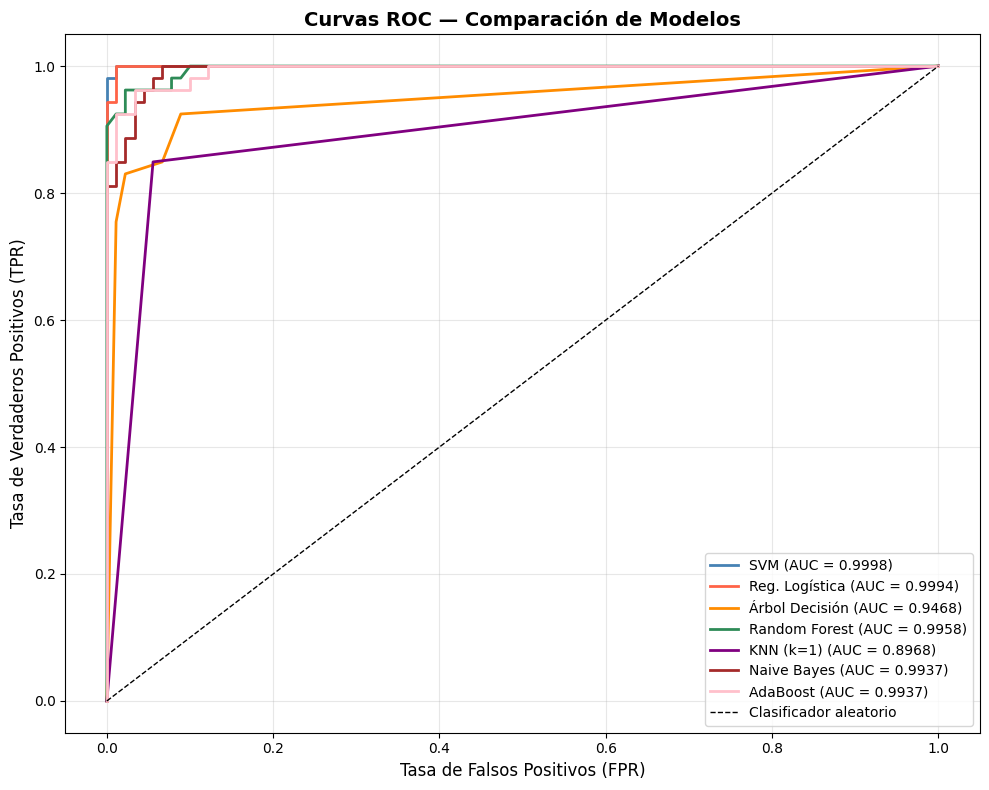
\includegraphics[width=\columnwidth]{images/fig_roc_curves.png}
  \caption{Curvas ROC para siete modelos (XGBoost y ANN no incluidos). Los valores de AUC oscilan entre 0.8968 (KNN) y 0.9998 (SVM), indicando la probabilidad de que el modelo asigne un \textit{score} más alto a una instancia maligna aleatoria que a una benigna aleatoria.}
  \label{fig:roc}
\end{figure}

\subsection{Ranking por métrica crítica}

La Tabla~\ref{tab:ranking} ordena los modelos por Recall Maligno, la métrica más relevante para el contexto clínico.

\begin{table}[!t]
\centering
\caption{Ranking por Recall Maligno ($\bigstar$ métrica crítica). AUC obtenido de curvas ROC (Fig.~\ref{fig:roc}); `---' indica modelo no incluido en esa figura.}
\label{tab:ranking}
\renewcommand{\arraystretch}{1.2}
\begin{tabular}{clccc}
\toprule
\textbf{Pos.} & \textbf{Modelo} & \textbf{Recall M.} & \textbf{Exactitud} & \textbf{AUC} \\
\midrule
1 & Regresión Logística & \cellcolor{verdemejor}\textbf{0.9434} & \textbf{0.9790} & 0.9994 \\
2 & XGBoost             & 0.9245 & 0.9650 & ---    \\
3 & SVM (lineal)        & 0.9057 & 0.9650 & \cellcolor{verdemejor}0.9998 \\
3 & ANN                 & 0.9057 & 0.9650 & ---    \\
3 & Random Forest       & 0.9057 & 0.9650 & 0.9958 \\
6 & AdaBoost            & 0.8679 & 0.9441 & 0.9937 \\
7 & Naive Bayes         & 0.8491 & 0.9371 & 0.9937 \\
7 & KNN ($k$=1)         & 0.8491 & 0.9091 & 0.8968 \\
9 & Árbol Decisión      & \cellcolor{rojomenor}0.8302 & 0.9231 & 0.9468 \\
\bottomrule
\end{tabular}
\end{table}

% ─── 8. ESTABILIDAD Y GENERALIZACIÓN ────────────────────────
\section{Estabilidad y Generalización de los Modelos}

La exactitud sobre un único conjunto de prueba puede ser
engañosa: un modelo puede obtener buenos resultados por azar
en una partición particular. La validación cruzada 5-fold
sobre el conjunto de entrenamiento estima el rendimiento
esperado en datos nuevos y cuantifica la varianza del modelo \cite{hastie2009}.
La Tabla~\ref{tab:cv} compara el Recall Maligno en el conjunto
de prueba con el CV Recall y su desviación estándar.

\begin{table}[!t]
\centering
\caption{Estabilidad de modelos: Recall Maligno en prueba vs.
validación cruzada 5-fold}
\label{tab:cv}
\renewcommand{\arraystretch}{1.25}
\begin{tabular}{lccc}
\toprule
\textbf{Modelo}
  & \textbf{\begin{tabular}[c]{@{}c@{}}Recall M.\\ (prueba)\end{tabular}}
  & \textbf{\begin{tabular}[c]{@{}c@{}}CV Recall\\ (media)\end{tabular}}
  & \textbf{\begin{tabular}[c]{@{}c@{}}CV Recall\\ ($\pm$ std)\end{tabular}} \\
\midrule
Reg. Logística  & \cellcolor{verdemejor}0.9434 & \cellcolor{verdemejor}0.9308 & 0.0247 \\
ANN             & 0.9057 & ---    & ---    \\
XGBoost         & 0.9245 & 0.8933 & \cellcolor{rojomenor}0.0464 \\
SVM (lineal)    & 0.9057 & 0.8933 & \cellcolor{rojomenor}0.0464 \\
Random Forest   & 0.9057 & 0.9183 & 0.0148 \\
AdaBoost        & 0.8679 & 0.8933 & 0.0313 \\
KNN ($k$=1)     & 0.8491 & 0.8990 & 0.0247 \\
Naive Bayes     & 0.8491 & 0.8804 & \cellcolor{verdemejor}0.0130 \\
Árbol Decisión  & \cellcolor{rojomenor}0.8302 & 0.8552 & 0.0388 \\
\bottomrule
\multicolumn{4}{l}{\parbox{\linewidth}{\small --- ANN excluida de CV: entrenamiento estocástico con Early Stopping no produce estimaciones comparables con modelos deterministas.}}
\end{tabular}
\end{table}

\textbf{Alta sensibilidad, alta estabilidad.} La Regresión
Logística lidera en solitario con Recall Maligno de 0.943
— casi cuatro puntos por encima del tercer bloque (0.906, formado
por SVM, ANN y RF) — y con una desviación moderada ($\pm$0.025).
Su ventaja sobre modelos más complejos confirma que el problema
es de naturaleza linealmente separable: la función sigmoide
captura la frontera de decisión con mayor eficiencia que una
red neuronal de 545 parámetros entrenada sobre 426 muestras.

\textbf{Alta sensibilidad, alta varianza.} XGBoost obtiene el
segundo mejor Recall Maligno (0.925) pero comparte con SVM la
mayor desviación estándar ($\pm$0.046). Esto indica que su
rendimiento es sensible a qué datos ve durante el entrenamiento,
un riesgo en datasets pequeños como el WDBC.

\textbf{Menor sensibilidad, mayor estabilidad.} Naive Bayes
presenta la desviación más baja de todos los modelos
($\pm$0.013), seguido de Random Forest ($\pm$0.015). Ambos
sacrifican algo de sensibilidad a cambio de predicciones
altamente consistentes entre particiones. Random Forest en
particular ofrece el mejor equilibrio entre rendimiento y
estabilidad de los métodos de ensemble.

La elección del modelo final depende del contexto
de uso: si se prioriza máxima detección de malignos,
la Regresión Logística es la opción; si se requiere robustez
ante variaciones en los datos de entrenamiento, Random Forest
es preferible; si se necesita interpretabilidad probabilística
para comunicar riesgo al paciente, Naive Bayes ofrece la mayor
consistencia con fundamento bayesiano explícito.
% ─── 9. DISCUSIÓN ────────────────────────────────────────────
\section{Discusión}

\subsection{Sobre el pipeline de analítica de datos}
La normalización z-score fue indispensable para SVM y KNN,
algoritmos sensibles a la escala al operar sobre distancias
euclidianas. La selección de atributos redujo la dimensionalidad
un 50\% (de 30 a 15 características) sin degradar el rendimiento
de los clasificadores, eliminando redundancias evidentes en el
mapa de correlación (Fig.~\ref{fig:heatmap}). La división
estratificada garantizó que el desbalance de clases (63\%/37\%)
se mantuviera igual en entrenamiento y prueba, evitando sesgos
en la evaluación.

\subsection{Sobre la métrica de evaluación}
Bajo accuracy, KNN ($k$=1) parece razonablemente competitivo
(90.9\%); bajo Recall Maligno, cae a los últimos puestos
(0.849, empatado con Naive Bayes) con 8 falsos negativos — 8 pacientes con cáncer que
recibirían un diagnóstico incorrecto. Esta diferencia ilustra
por qué en problemas médicos con desbalance de clases la
accuracy no es una métrica suficiente \cite{hossin2015, sokolova2009}.

De forma análoga, SVM y Random Forest comparten exactamente
las mismas métricas puntuales, pero su análisis de estabilidad revela que Random Forest
es tres veces más estable en validación cruzada
($\pm$0.015 vs $\pm$0.046). Una evaluación basada únicamente
en el conjunto de prueba habría concluido que ambos modelos
son equivalentes, ocultando una diferencia operacionalmente
relevante.

KNN presenta además la mayor
brecha entre el Recall en prueba (0.849) y el CV Recall (0.899)
— una diferencia de 0.050 puntos, la más amplia del experimento.
Esto indica que el conjunto de prueba resultó especialmente
desfavorable para KNN, lo que hace su rendimiento puntual
menos representativo que el de los demás modelos. En un
contexto clínico, esta sensibilidad a la partición de datos
es un riesgo adicional frente a modelos más estables.

\subsection{Sobre la elección del modelo}
Las diferencias de Recall entre modelos son pequeñas en valor
absoluto: la distancia entre el primero (LR, 0.943) y el tercero
(SVM/RF/ANN, 0.906) corresponde a 2 predicciones sobre 53 instancias
malignas. Con el IC de Wilson al 95\% para LR de $[0.85,\,0.98]$,
parte del ranking observado puede ser ruido muestral. Las
siguientes hipótesis de uso deben entenderse como orientación
para diseño de estudios futuros con validación externa, no como
directrices de despliegue:

\begin{itemize}
  \item \textbf{Screening masivo} (prioridad: sensibilidad):
  Regresión Logística — mayor Recall Maligno (0.943) con
  precisión perfecta (1.000) y coeficientes auditables.

  \item \textbf{Robustez ante variaciones en los datos}:
  Random Forest — mejor estabilidad en CV ($\pm$0.015) con
  rendimiento competitivo.

  \item \textbf{Cuantificación de incertidumbre}:
  Naive Bayes Gaussiano — probabilidades posteriores
  $P(\text{Maligno}|\mathbf{x})$ con la menor varianza
  en CV ($\pm$0.013).

  \item \textbf{Balance rendimiento/costo computacional}:
  XGBoost — segundo mejor Recall Maligno (0.925); su CV std
  elevado ($\pm$0.046) requiere atención ante variaciones en
  los datos de entrenamiento.

  \item \textbf{Interpretabilidad para personal médico}:
  Árbol de Decisión — reglas SI–ENTONCES auditables, con el
  menor Recall Maligno del conjunto (0.830).
\end{itemize}

\subsection{Limitaciones}
\begin{itemize}
  \item El dataset proviene de un único centro médico
  (Universidad de Wisconsin), lo que puede limitar la
  generalización a otras poblaciones, equipos de imagen
  o protocolos de FNA.

  \item El tamaño reducido (569 instancias) limita la
  potencia estadística de la comparación y es insuficiente
  para arquitecturas de \textit{deep learning} más complejas \cite{chougrad2018}.

  \item El análisis se realiza sobre características
  morfológicas extraídas automáticamente; no incorpora
  factores de riesgo clínicos (edad, historial familiar,
  marcadores genéticos) que en la práctica son determinantes.

  \item La validación es interna (split train/test con
  semilla fija). Una validación externa sobre un dataset
  independiente de otro centro médico permitiría estimar la generalización a poblaciones, equipos de imagen y protocolos de FNA distintos \cite{hastie2009}.

  \item La ANN no fue incluida en la validación cruzada;
  su entrenamiento estocástico con Early Stopping produce
  estimaciones de CV no comparables directamente con los
  modelos deterministas.

  \item No se aplicaron pruebas de significancia estadística
  pareadas entre clasificadores (p.\,ej.\ la prueba de
  McNemar para la exactitud o la prueba de DeLong para el
  AUC). Dado el tamaño reducido del conjunto de prueba
  (53 instancias malignas), los intervalos de confianza
  de las métricas son amplios: el Recall Maligno de la
  Regresión Logística (0.943) tiene un intervalo de
  confianza de Wilson al 95\% de aproximadamente
  $[0.85,\,0.98]$. En consecuencia, algunas diferencias
  de ranking entre modelos cercanos podrían no ser
  estadísticamente significativas; su contraste formal
  queda como trabajo futuro \cite{sokolova2009}.
\end{itemize}

% ─── 10. CONCLUSIONES ────────────────────────────────────────
\section{Conclusiones}

Se implementó un pipeline completo de analítica de datos para la detección de cáncer de mama. A continuación se presentan las conclusiones organizadas por cada fase del pipeline:

\subsection{Fase de Análisis Exploratorio (EDA)}
El análisis exploratorio reveló bloques de alta correlación entre las versiones \textit{mean}, \textit{error} y \textit{worst} de los mismos atributos morfológicos, evidenciando redundancia significativa en el espacio original de 30 características. La visualización de distribuciones por clase permitió identificar visualmente los atributos con mayor poder discriminativo (\texttt{mean area}, \texttt{mean concavity}), orientando las decisiones posteriores de selección de atributos.

\subsection{Fase de Preprocesamiento}
La \textbf{normalización z-score} fue indispensable para el correcto funcionamiento de SVM y KNN, algoritmos sensibles a la escala de los datos \cite{kantardzic, garcia2015}. La aplicación correcta del escalador (\texttt{fit} solo en train) evitó el \textit{data leakage}, un error metodológico que habría inflado artificialmente las métricas de evaluación. La decisión de conservar los valores anómalos (13\% de las instancias) fue validada por los resultados: eliminarlos habría reducido la capacidad del modelo para detectar tumores atípicos, que son precisamente los casos más críticos.

\subsection{Fase de Selección de Atributos}
La \textbf{selección por intersección de dos métodos} (correlación con la variable objetivo y prueba de separación de medias) redujo las características de 30 a 15 (50\% de reducción) manteniendo el rendimiento competitivo de los clasificadores \cite{remeseiro2019}. Las 15 características descartadas correspondieron a atributos con bajo poder discriminativo (\textit{texture}, \textit{smoothness}, \textit{symmetry}, \textit{fractal dimension}), confirmando lo observado en el EDA. La convergencia de ambos métodos sobre el mismo subconjunto respalda la relevancia de las características seleccionadas, aunque el criterio de correlación fue el determinante del resultado final.

\subsection{Fase de Modelado}
La \textbf{Regresión Logística} obtuvo el mayor Recall Maligno (94.34\%) con precisión perfecta (1.000, cero falsos positivos), la mejor combinación para screening clínico. Que un modelo lineal supere a SVM, Random Forest y ANN en sensibilidad (estos tres igualados en 90.57\%) indica que el problema es linealmente separable con las 15 características seleccionadas: la mayor capacidad de los métodos complejos no aporta ventaja en este caso. El \textbf{Naive Bayes Gaussiano}, basado en la Teoría Bayesiana \cite{bayesian_med}, entrega probabilidades posteriores explícitas $P(\text{Maligno} | \mathbf{x})$ que cuantifican la incertidumbre del diagnóstico.

\subsection{Fase de Evaluación}
La métrica de \textbf{accuracy es insuficiente} para problemas médicos con desbalance de clases \cite{hossin2015, sokolova2009}. KNN obtuvo 90.9\% de accuracy pero solo 84.91\% de Recall Maligno, dejando 8 tumores malignos sin detectar. El uso conjunto de Recall, Precisión, F1 y AUC-ROC permite una evaluación más completa y honesta del rendimiento del clasificador. La priorización del Recall Maligno como métrica principal fue determinante para identificar a la Regresión Logística como el mejor modelo, un resultado que el accuracy por sí solo habría ocultado.

\subsection{Fase de Estabilidad y Generalización}
La \textbf{validación cruzada 5-fold} \cite{hastie2009} permitió distinguir entre modelos con alto rendimiento puntual pero inestable (XGBoost, SVM con $\pm$0.046 de desviación) y modelos más robustos (Random Forest con $\pm$0.015, Naive Bayes con $\pm$0.013). La Regresión Logística combina el mejor rendimiento puntual con estabilidad moderada ($\pm$0.025), confirmando su idoneidad como modelo de referencia. La elección del modelo final no depende únicamente de las métricas puntuales, sino del contexto de uso: screening masivo, segunda opinión clínica o comunicación de riesgo al paciente requieren perfiles distintos de sensibilidad y estabilidad.

\subsection{Conclusión General}
Los resultados muestran que la selección de métricas y el preprocesamiento son tan determinantes como el algoritmo: la Regresión Logística supera a modelos más complejos —SVM, Random Forest, ANN— no por mayor capacidad, sino porque el problema es linealmente separable con las 15 características seleccionadas, y el Recall Maligno como métrica principal expone diferencias que la exactitud oculta \cite{hossin2015, sokolova2009}. El siguiente paso para sustentar estas conclusiones con mayor certeza estadística es aplicar tests pareados (McNemar, DeLong) y validar sobre un dataset externo independiente \cite{hastie2009}.

% ─── REFERENCIAS ─────────────────────────────────────────────
\begin{thebibliography}{27}

\bibitem{who2023}
World Health Organization, ``Breast cancer,'' WHO Fact Sheets, 2023. [En línea]. Disponible: \url{https://www.who.int/news-room/fact-sheets/detail/breast-cancer}

\bibitem{sung2021}
H. Sung et al., ``Global Cancer Statistics 2020: GLOBOCAN Estimates of Incidence and Mortality Worldwide for 36 Cancers in 185 Countries,'' \textit{CA: A Cancer Journal for Clinicians}, vol. 71, no. 3, pp. 209--249, 2021.

\bibitem{wdbc1993}
W. H. Wolberg, W. N. Street, y O. L. Mangasarian, ``Breast Cancer Wisconsin (Diagnostic),'' UCI Machine Learning Repository, 1993. DOI: \url{https://doi.org/10.24432/C5DW2B}

\bibitem{bayesian_med}
J. Rodríguez y L. González, ``Prototipo de software para la clasificación de datos mediante el método bayesiano TAN -- UDTan,'' \textit{Visión Electrónica}, vol. 11, no. 2, 2017.

\bibitem{curso_ud}
J. E. Rodríguez, \textit{Fundamentos de Minería de Datos}. Bogotá: Fondo de publicaciones Universidad Distrital Francisco José de Caldas, 2010.

\bibitem{svm_vapnik}
V. Vapnik, \textit{The Nature of Statistical Learning Theory}. New York: Springer, 1995.

\bibitem{rna_ud}
J. Hilera y V. Martínez, \textit{Redes Neuronales Artificiales: Fundamentos, Modelos y Aplicaciones}. Madrid: RA-MA, 1995.

\bibitem{feature_sel}
V. H. Medina G. y J. E. Rodríguez R., ``A comparative study between feature selection algorithms,'' Trabajo de investigación, Universidad Distrital Francisco José de Caldas, Bogotá, Colombia, 2017.

\bibitem{kantardzic}
M. Kantardzic, \textit{Data Mining: Concepts, Models, Methods and Algorithms}, 2nd ed. IEEE Press Wiley-Interscience, 2003.

\bibitem{cac2024}
Cuenta de Alto Costo, ``Día mundial del cáncer de mama --- Situación del cáncer de mama en Colombia,'' Oct. 2024. [En línea]. Disponible: \url{https://cuentadealtocosto.org/noticias/dia-mundial-del-cancer-de-mama/}

\bibitem{elmore2015}
J. G. Elmore et al., ``Diagnostic Concordance Among Pathologists Interpreting Breast Biopsy Specimens,'' \textit{JAMA}, vol. 313, no. 11, pp. 1122--1132, 2015.

\bibitem{kourou2015}
K. Kourou, T. P. Exarchos, K. P. Exarchos, M. V. Karamouzis, y D. I. Fotiadis, ``Machine learning applications in cancer prognosis and prediction,'' \textit{Computational and Structural Biotechnology Journal}, vol. 13, pp. 8--17, 2015.

\bibitem{asri2016}
H. Asri, H. Mousannif, H. Al Moatassime, y T. Noel, ``Using Machine Learning Algorithms for Breast Cancer Risk Prediction and Diagnosis,'' \textit{Procedia Computer Science}, vol. 83, pp. 1064--1069, 2016.

\bibitem{remeseiro2019}
B. Remeseiro y V. Bolon-Canedo, ``A review of feature selection methods in medical applications,'' \textit{Computers in Biology and Medicine}, vol. 112, art. 103375, 2019.

\bibitem{breiman2001}
L. Breiman, ``Random Forests,'' \textit{Machine Learning}, vol. 45, no. 1, pp. 5--32, 2001.

\bibitem{chen2016}
T. Chen y C. Guestrin, ``XGBoost: A Scalable Tree Boosting System,'' en \textit{Proceedings of the 22nd ACM SIGKDD International Conference on Knowledge Discovery and Data Mining}, pp. 785--794, 2016.

\bibitem{hastie2009}
T. Hastie, R. Tibshirani, y J. Friedman, \textit{The Elements of Statistical Learning: Data Mining, Inference, and Prediction}, 2nd ed. New York: Springer, 2009.

\bibitem{pedregosa2011}
F. Pedregosa et al., ``Scikit-learn: Machine Learning in Python,'' \textit{Journal of Machine Learning Research}, vol. 12, pp. 2825--2830, 2011.

\bibitem{chollet2015}
F. Chollet, ``Keras,'' GitHub, 2015. [En línea]. Disponible: \url{https://github.com/fchollet/keras}

\bibitem{hossin2015}
M. Hossin y M. N. Sulaiman, ``A Review on Evaluation Metrics for Data Classification Evaluations,'' \textit{International Journal of Data Mining \& Knowledge Management Process}, vol. 5, no. 2, pp. 1--11, 2015.

\bibitem{sokolova2009}
M. Sokolova y G. Lapalme, ``A systematic analysis of performance measures for classification tasks,'' \textit{Information Processing \& Management}, vol. 45, no. 4, pp. 427--437, 2009.

\bibitem{chougrad2018}
H. Chougrad, H. Zouaki, y O. Alheyane, ``Deep Convolutional Neural Networks for breast cancer screening,'' \textit{Computer Methods and Programs in Biomedicine}, vol. 157, pp. 19--30, 2018.

\bibitem{garcia2015}
S. García, J. Luengo, y F. Herrera, \textit{Data Preprocessing in Data Mining}. Cham: Springer, 2015.

\bibitem{freund1997}
Y. Freund y R. E. Schapire, ``A decision-theoretic generalization of on-line learning and an application to boosting,'' \textit{Journal of Computer and System Sciences}, vol. 55, no. 1, pp. 119--139, 1997.

\bibitem{strelcenia2023}
E. Strelcenia y S. Prakoonwit, ``Effective Feature Engineering and Classification of Breast Cancer Diagnosis: A Comparative Study,'' \textit{BioMedInformatics}, vol. 3, no. 3, pp. 616--631, 2023.

\bibitem{rajpoot2024}
C. S. Rajpoot, G. Sharma, P. Gupta, P. Dadheech, U. Yahya, y N. Aneja, ``Feature Selection-based Machine Learning Comparative Analysis for Predicting Breast Cancer,'' \textit{Applied Artificial Intelligence}, vol. 38, no. 1, art. 2340386, 2024.

\bibitem{domingos1997}
P. Domingos y M. Pazzani, ``On the Optimality of the Simple Bayesian Classifier under Zero-One Loss,'' \textit{Machine Learning}, vol. 29, no. 2--3, pp. 103--130, 1997.

\end{thebibliography}

\end{document}
